%%%%%%%%%%%%%%%%%%%%%%%%%%%%%%%%%%%%%%%%%
% Beamer Presentation
% LaTeX Template
% Version 1.0 (10/11/12)
%
% This template has been downloaded from:
% http://www.LaTeXTemplates.com
%
% License:
% CC BY-NC-SA 3.0 (http://creativecommons.org/licenses/by-nc-sa/3.0/)
%
%%%%%%%%%%%%%%%%%%%%%%%%%%%%%%%%%%%%%%%%%

%----------------------------------------------------------------------------------------
%	PACKAGES AND THEMES
%----------------------------------------------------------------------------------------
\documentclass{beamer}

\mode<presentation> {

% The Beamer class comes with a number of default slide themes
% which change the colors and layouts of slides. Below this is a list
% of all the themes, uncomment each in turn to see what they look like.

\usetheme{CambridgeUS}

% As well as themes, the Beamer class has a number of color themes
% for any slide theme. Uncomment each of these in turn to see how it
% changes the colors of your current slide theme.

%\usecolortheme{albatross}
%\usecolortheme{beaver}
%\usecolortheme{beetle}
%\usecolortheme{crane}
%\usecolortheme{dolphin}
%\usecolortheme{dove}
%\usecolortheme{fly}
%\usecolortheme{lily}
%\usecolortheme{orchid}
%\usecolortheme{rose}
%\usecolortheme{seagull}
%\usecolortheme{seahorse}
%\usecolortheme{whale}
%\usecolortheme{wolverine}

%\setbeamertemplate{footline} % To remove the footer line in all slides uncomment this line
%\setbeamertemplate{footline}[page number] % To replace the footer line in all slides with a simple slide count uncomment this line

%\setbeamertemplate{navigation symbols}{} % To remove the navigation symbols from the bottom of all slides uncomment this line
}
%----------------------------------------------------------------------------------------
\usepackage{graphicx} % Allows including images
\usepackage{booktabs} % Allows the use of \toprule, \midrule and \bottomrule in tables
\setbeamerfont{caption}{size=\scriptsize}
\usepackage{hyperref}
\usepackage{listings} % for code listings
\lstset{
  language={C++},
  basicstyle=\footnotesize
}
\usepackage{marvosym} % for smileys

%----------------------------------------------------------------------------------------
%	TITLE PAGE
%----------------------------------------------------------------------------------------
\title[]{Arduino in der Robotik} % The short title appears at the bottom of every slide, the full title is only on the title page
%----------------------------------------------------------------------------------------
\author{Alexander Entinger} % Your name
\institute{LXRobotics GmbH}
\date{\today} % Date, can be changed to a custom date
%----------------------------------------------------------------------------------------
\begin{document}
%----------------------------------------------------------------------------------------
\section{Arduino in der Robotik}
%----------------------------------------------------------------------------------------
\begin{frame}
\titlepage % Print the title page as the first slide
\end{frame}
%%----------------------------------------------------------------------------------------
%%	PRESENTATION SLIDES
%%----------------------------------------------------------------------------------------
\begin{frame}{Alexander Entinger}
\begin{itemize}
 \item CEO/CTO LXRobotics
  \begin{figure}[H]
   \centering
   
\includegraphics[width=0.3\textwidth]{./images/logo-lxrobotics.png}
   \label{fig:logo-lxrobotics}
  \end{figure}
\end{itemize}
\begin{itemize}
 \item Embedded Software Developer DS Automotion
  \begin{figure}[H]
   \centering
   
\includegraphics[width=0.3\textwidth]{./images/logo-ds-automotion.jpg}
   \label{fig:logo-ds-automotion}
  \end{figure}
\end{itemize}
\begin{itemize}
 \item Projektbetreuer Robotik Fachhochschule Hagenberg
 \begin{itemize}
  \item Masterstudiengang Embedded Systems Design
 \end{itemize}
   \begin{figure}[H]
    \centering
    
\includegraphics[width=0.3\textwidth]{./images/logo-fh-hagenberg.png}
    \label{fig:logo-fh-hagenberg}
   \end{figure}
\end{itemize}
\end{frame}
%%----------------------------------------------------------------------------------------
\begin{frame}{Alexander Entinger - Roboter (1)}
	\begin{columns}
		\begin{column}{0.5\textwidth}
			\begin{large}Mini Sumo Roboter \textbf{Sergeant Pain}\end{large}
			\begin{itemize}
				\item Robotchallenge 2011
			\end{itemize}
		\end{column}
		\begin{column}{0.5\textwidth}
			\begin{figure}[H]
				\centering
				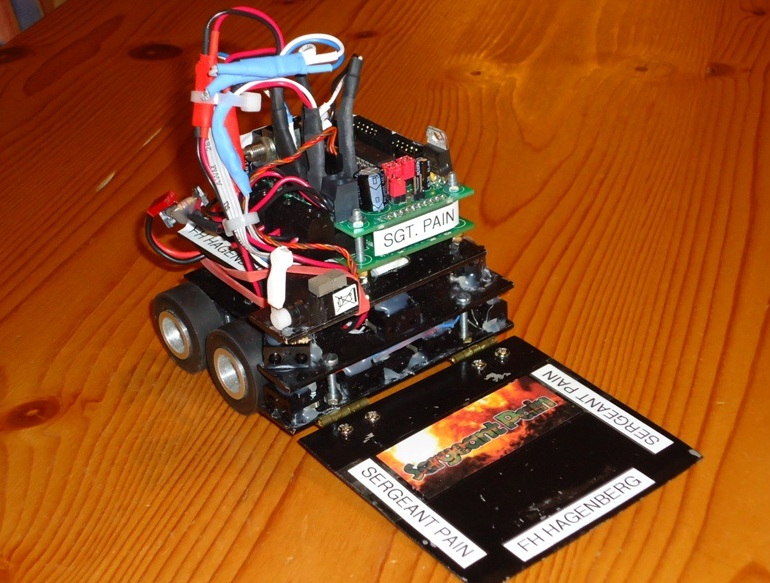
\includegraphics[width=0.7\textwidth]{./images/robot-sergeant-pain.jpg}
				\label{fig:robot-sergeant-pain}
			\end{figure}
		\end{column}
	\end{columns}
	
	\begin{columns}
		\begin{column}{0.5\textwidth}
			\begin{large}Mini Sumo Roboter \textbf{Evolution}\end{large}
			\begin{itemize}
				\item Robotchallenge 2014
			\end{itemize}
		\end{column}
		\begin{column}{0.5\textwidth}
			\begin{figure}[H]
				\centering
				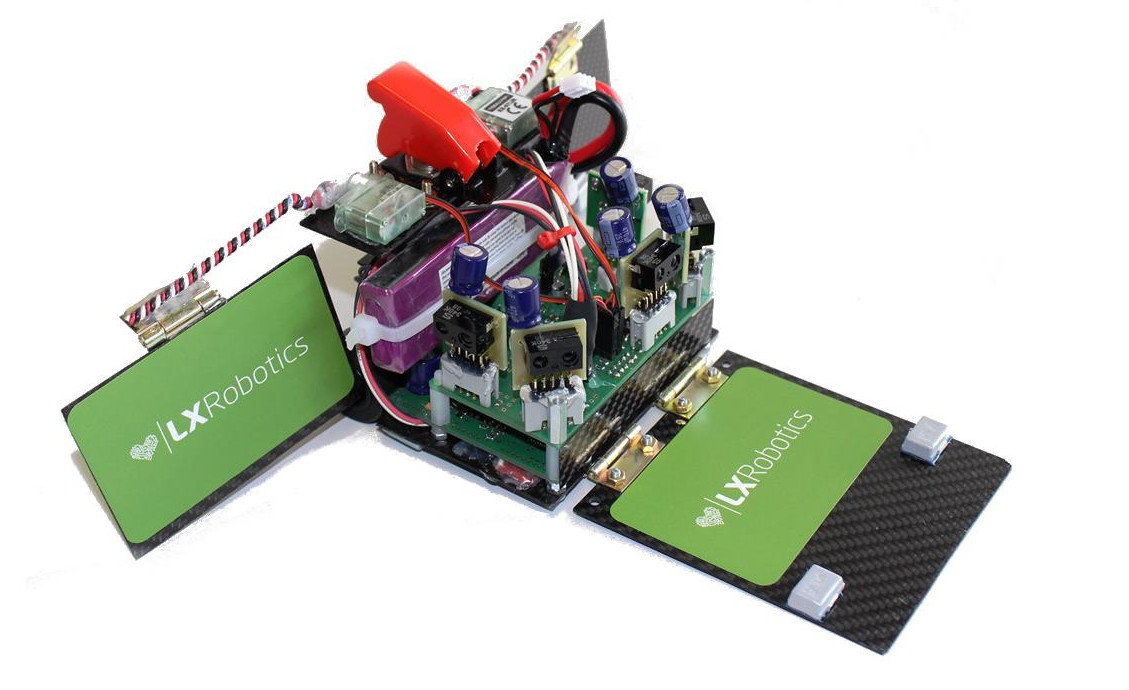
\includegraphics[width=0.7\textwidth]{./images/robot-evolution.jpg}
				\label{fig:robot-evolution}
			\end{figure}
		\end{column}
	\end{columns}
\end{frame}
%%----------------------------------------------------------------------------------------
\begin{frame}{Alexander Entinger - Roboter (2)}
	\begin{columns}
		\begin{column}{0.5\textwidth}
			\begin{large}Featherweight \textbf{Schnauzer}\end{large}
			\begin{itemize}
				\item 1. Platz Mad Metal Machines Vol. 19 / Bochum / DE
				\item 1. Platz European Robotcombat Cup 2015
			\end{itemize}
		\end{column}
		\begin{column}{0.5\textwidth}
			\begin{figure}[H]
				\centering
				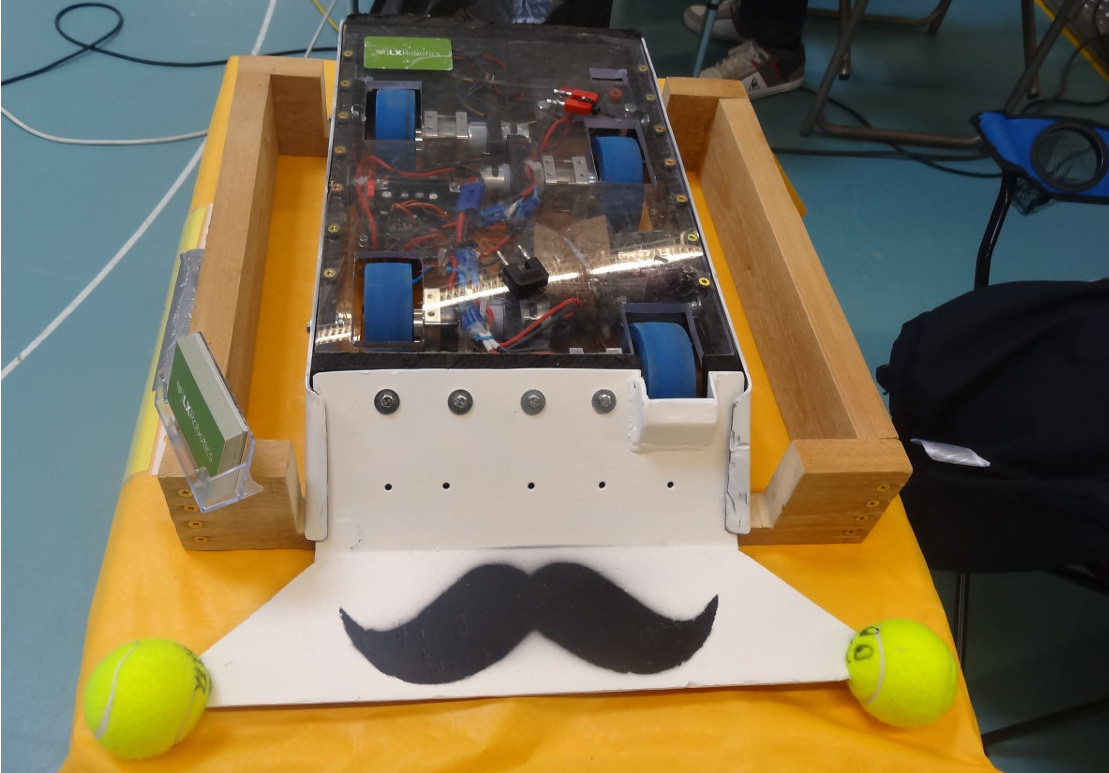
\includegraphics[width=0.7\textwidth]{./images/robot-schnauzer.jpg}
				\label{fig:robot-schnauzer}
			\end{figure}
		\end{column}
	\end{columns}
	
	\begin{columns}
		\begin{column}{0.5\textwidth}
			\begin{large}Featherweight \textbf{Steroid}\end{large}
		\end{column}
		\begin{column}{0.5\textwidth}
			\begin{figure}[H]
				\centering
				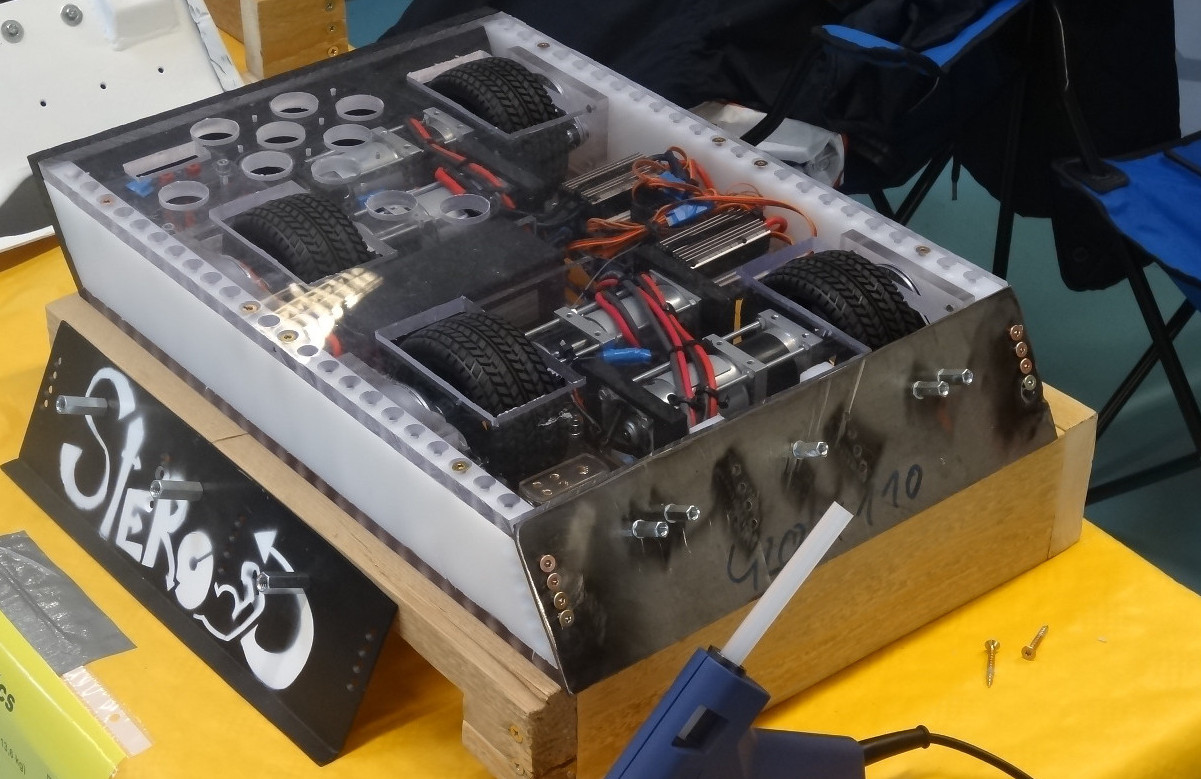
\includegraphics[width=0.7\textwidth]{./images/robot-steroid.jpg}
				\label{fig:robot-steroid}
			\end{figure}
		\end{column}
	\end{columns}
\end{frame}
%%----------------------------------------------------------------------------------------
\begin{frame}{Alexander Entinger - Roboter (3)}
	\begin{columns}
		\begin{column}{0.5\textwidth}
			\begin{large}ROS enabled SLAM Demonstrator \textbf{Beauty Queen}\end{large}
			\begin{itemize}
				\item Masterarbeitsprojekt (2012/13)
			\end{itemize}
		\end{column}
		\begin{column}{0.5\textwidth}
			\begin{figure}[H]
				\centering
				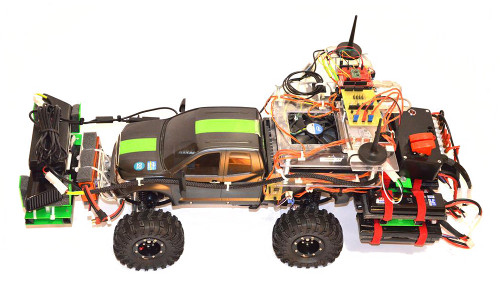
\includegraphics[width=0.7\textwidth]{./images/robot-beauty-queen.jpg}
				\label{fig:robot-beauty-queen}
			\end{figure}
		\end{column}
	\end{columns}
	
	\begin{columns}
		\begin{column}{0.5\textwidth}
			\begin{large}Hexapod \textbf{Lex}\end{large}
		\end{column}
		\begin{column}{0.5\textwidth}
			\begin{figure}[H]
				\centering
				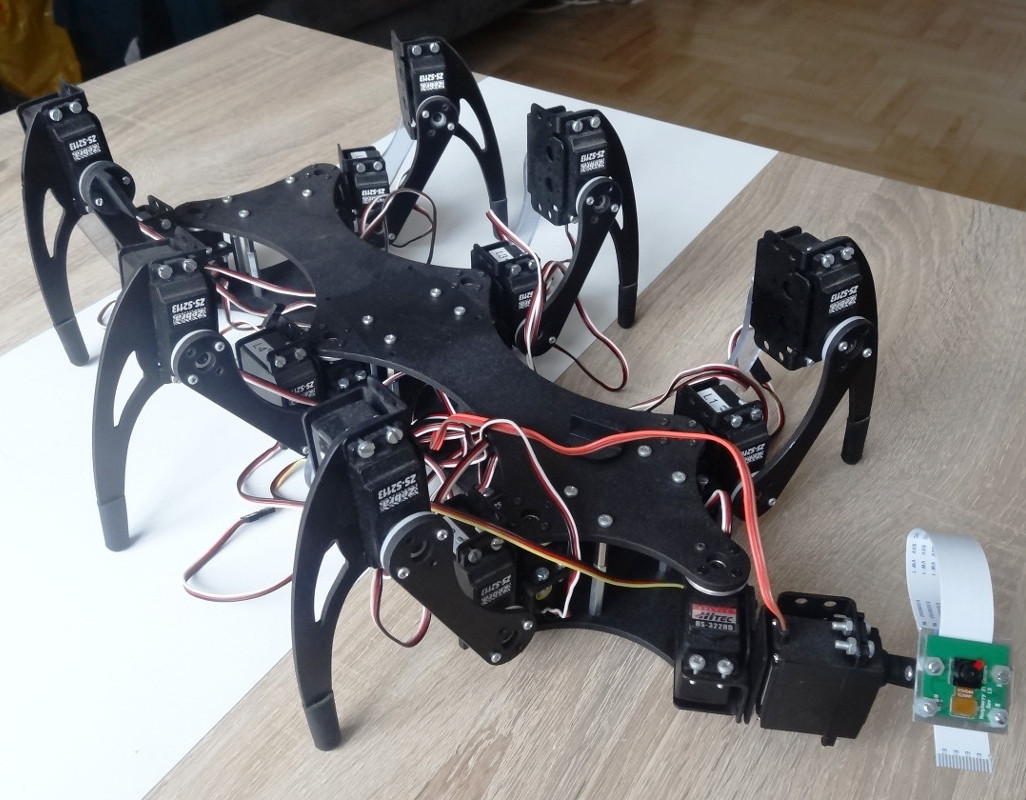
\includegraphics[width=0.7\textwidth]{./images/robot-lex.jpg}
				\label{fig:robot-lex}
			\end{figure}
		\end{column}
	\end{columns}
\end{frame}
%%----------------------------------------------------------------------------------------
\begin{frame}{Was haben alle diese Roboter gemeinsam?}
\begin{figure}[H]
	\centering
	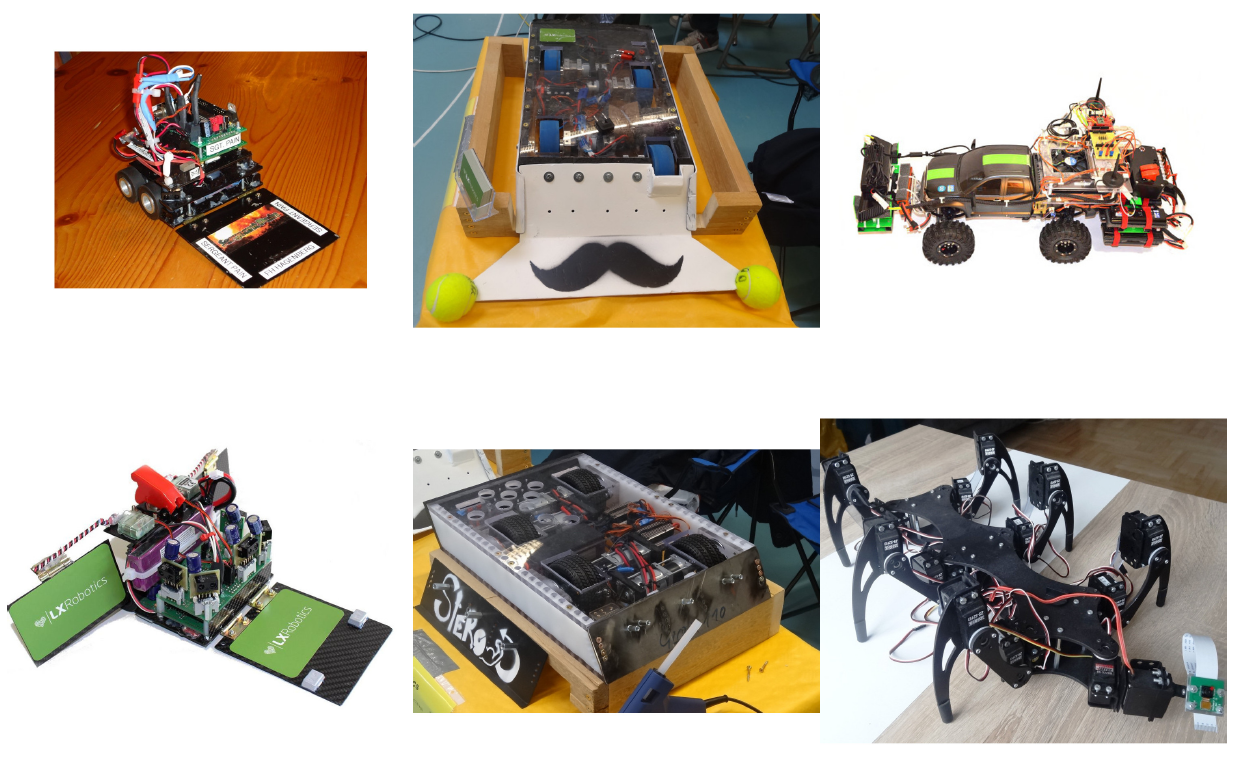
\includegraphics[width=1.0\textwidth]{./images/robots-all.png}
\end{figure}
\end{frame}
%%----------------------------------------------------------------------------------------
\begin{frame}{Was haben alle diese Roboter gemeinsam?}
	\begin{figure}[H]
		\centering
		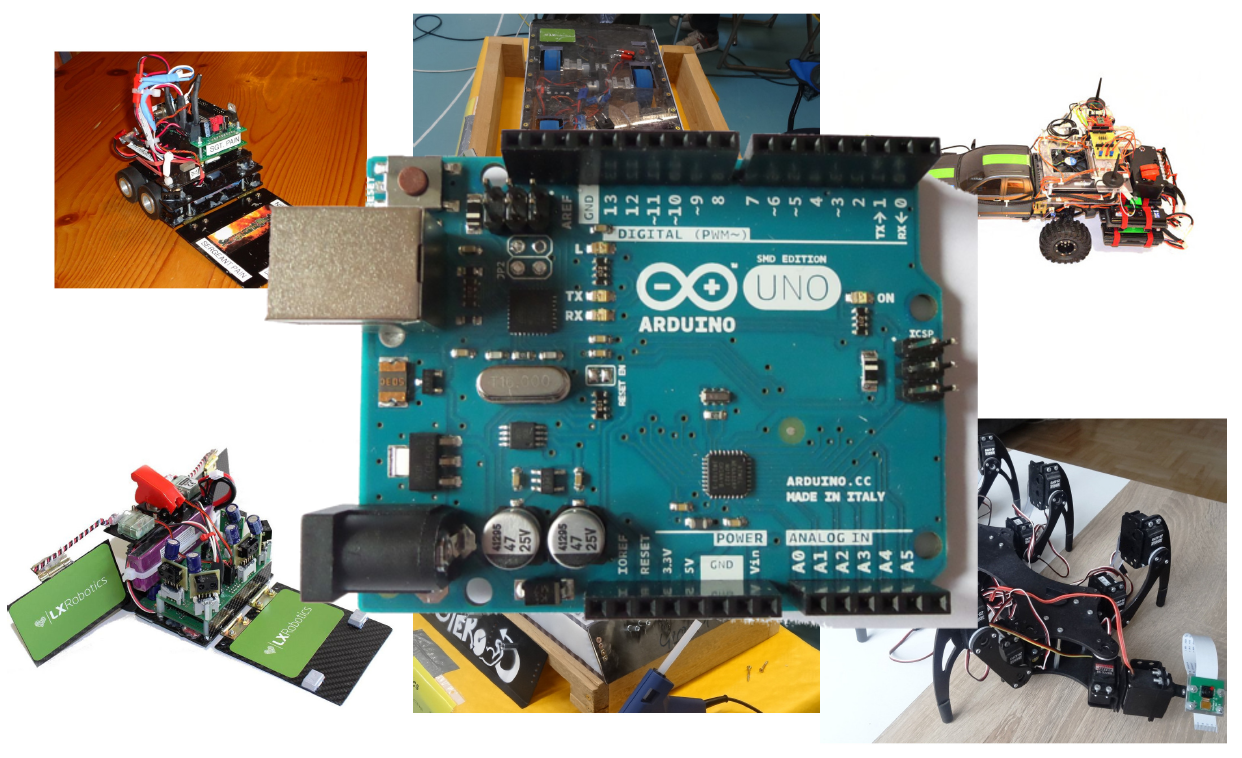
\includegraphics[width=1.0\textwidth]{./images/robots-all-arduino.png}
	\end{figure}
\end{frame}
%%----------------------------------------------------------------------------------------
\begin{frame}{Die Anf\"ange von Arduino (1)}
\begin{itemize}
	 \item Entwicklung des Arduino Konzepts durch \textbf{Massimo Banzi} und \textbf{David Cuartielles}\footnote{Weitere Teammitglieder: Tom Igoe, Gianluca Martino, David Mellis\cite{IEEE:2016:TheMakingOfArduino}\\}
\end{itemize}
\begin{itemize}
	\item \textbf{Hintergrund}: Banzi war als \textbf{Associate Professor} bei dem \textbf{Interaction Design Institute Ivrea} (Italien) f\"ur die \textbf{Physical Computing} Projekte verantwortlich.
\end{itemize}
\begin{alertblock}{Physical Computing ...}
	... bezeichnet ein aus Hard- und Softwarekomponenten bestehendes System, welches mit der analogen Welt interagiert.
\end{alertblock}
\end{frame}
%%----------------------------------------------------------------------------------------
\begin{frame}{Die Anf\"ange von Arduino (2)}
\begin{columns}
	\begin{column}{0.7\textwidth}
	\begin{itemize}
		\item Bisherige Plattform f\"ur Physical Computing am IDII: \textbf{BASIC Stamp}
		\begin{itemize}
			\item \textbf{PIC} basierte $\mu{}$C-Board mit integriertem BASIC-Interpreter
			\item Nachteile:
			\begin{itemize}
				\item Teuer ($\approx$ 100 \$)
				\item Nicht f\"ur alle Projekte ausreichende Rechenleistung
			\end{itemize}
		\end{itemize}
	\end{itemize}
	\end{column}
	\begin{column}{0.3\textwidth}
		\begin{figure}[H]
			\centering
			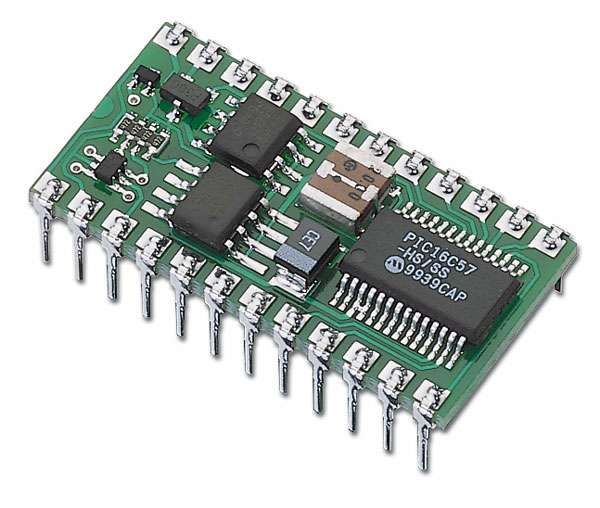
\includegraphics[width=1.0\textwidth]{./images/basic-stamp.jpg}
			\label{fig:basic-stamp}
			\caption{BASIC Stamp\cite{Image:BasicSTAMP}}
		\end{figure}
	\end{column}
\end{columns}
\vspace{20px}
\begin{itemize}
	\item \textbf{Konsequenz:} Konzeption der aus \textbf{Hard- und Software}komponenten bestehenden \textbf{Arduino Plattform} in 2005
\end{itemize}
\end{frame}
%%----------------------------------------------------------------------------------------
\begin{frame}{Arduino Plattform: Hardware}
\begin{columns}
 \begin{column}{0.7\textwidth}
 \begin{itemize}
  \item Kosteng\"unstige $\mu$C-Boards auf Basis von (zumeist 8-Bit) ATMEL Prozessoren
  \begin{itemize}
  	\item I/Os werden auf Buchsenleisten herausgef\"uhrt $\rightarrow$ einfacher Anschluss von Sensoren/Aktoren m\"oglich
  	\item Schaltplan/Layout werden unter permissiver \textbf{Creative Commons Attribution Share-Alike} Lizenz freigegeben
  \end{itemize}
 \end{itemize}
 \begin{itemize}
  \item Arbeitspferd: \textbf{Arduino Uno} (ATMega328) ($\approx$ 20 \EUR{}) 
 \end{itemize}
 \end{column}
 \begin{column}{0.3\textwidth}
  \begin{figure}[H]
   \centering
   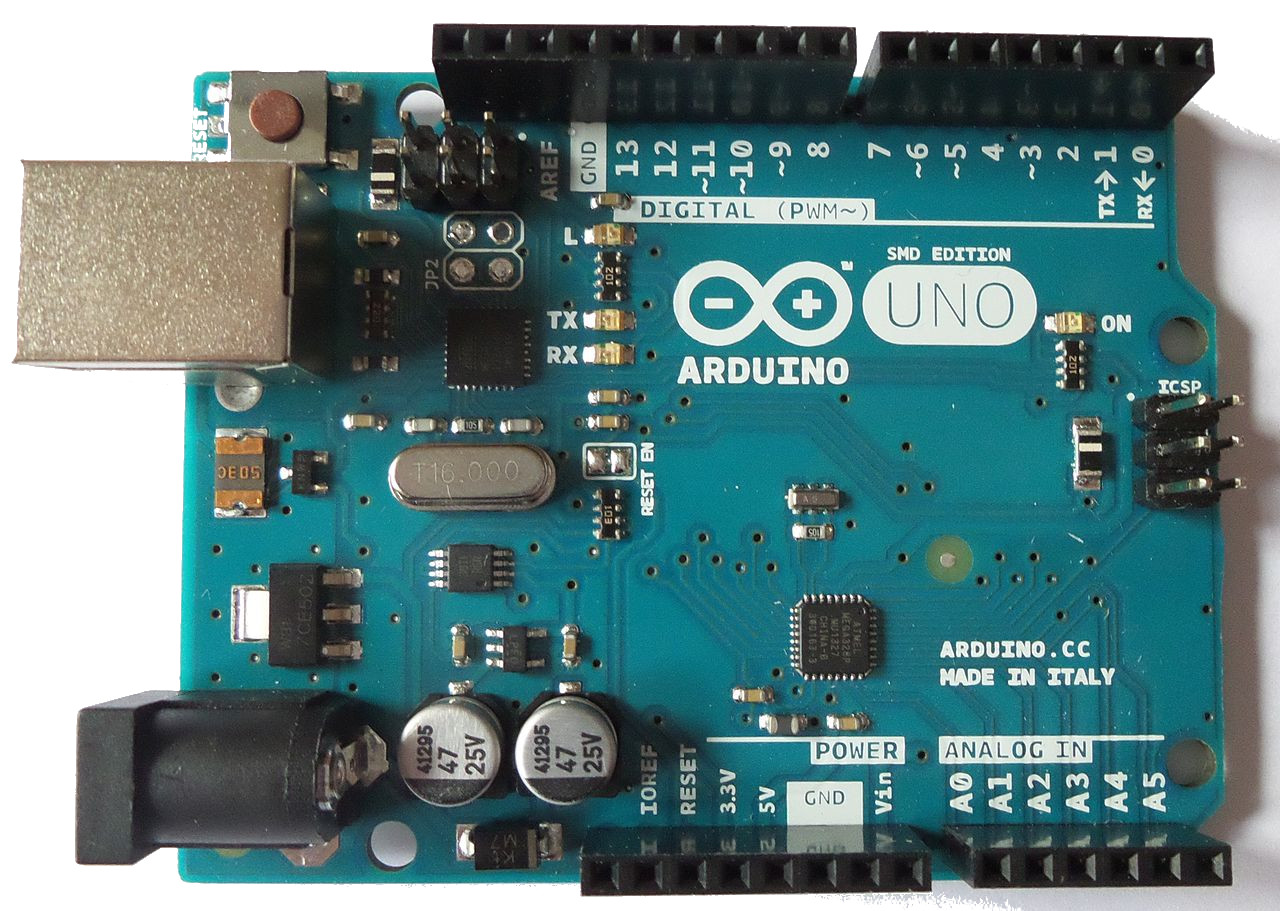
\includegraphics[width=0.9\textwidth]{./images/arduino-uno.jpg}
   \label{fig:arduino-uno}
   \caption{Arduino Uno\cite{Image:ArduinoUno}}
  \end{figure}
 \end{column}
\end{columns}
 \begin{itemize}
 	\item Weitere Arduinos:
 	\begin{itemize}
 		\item ATMega168: \textbf{Diecimila/Duemilanove}
 		\item ATMega32U4: \textbf{Leonardo}
 		\item ATMega2560: \textbf{Mega} 
 		\item SAM3X8E (32 Bit Cortex-M3): \textbf{Due}
 		\item ...
 	\end{itemize}
 \end{itemize}
\end{frame}
%%----------------------------------------------------------------------------------------
\begin{frame}[fragile]{Arduino Plattform: Software (1)}
\begin{itemize}
	\item Kostenlose Open Source (GPL) \textbf{Arduino-IDE} (Java)
\end{itemize}
\begin{itemize}
	\item Komplexes Thema der Embedded Programmierung wird durch Software-Framework stark vereinfacht
	\begin{itemize}
	 	\item \textbf{Nur 2 Funktionen:}
	 	\begin{itemize}
	 		\item \textbf{setup} $\rightarrow$ wird beim Start einmalig ausgef\"uhrt
	 		\item \textbf{loop} $\rightarrow$ wird kontinuierlich ausgef\"uhrt
	 	\end{itemize}
	 \end{itemize}
\end{itemize}
\begin{lstlisting}[frame=single, language=C]
void setup()
{
  pinMode(ledPin, OUTPUT);
}
void loop()
{
  digitalWrite(ledPin, HIGH);
  ...
}
\end{lstlisting}
\end{frame}
%%----------------------------------------------------------------------------------------
\begin{frame}[fragile]{Arduino Plattform: Software (2)}
\begin{itemize}
 	\item $\mu$C-Bibliotheken (LGPL) erm\"oglichen Hardware-Zugriff \"uber \textbf{abstrakte High-Level Befehle} ohne Detail-Kenntnisse der Interna des verwendeten $\mu$Cs
\end{itemize}
\begin{lstlisting}[frame=single, language=C]
/* I/O (Digital/Analog) */
int const buttonVal = digitalRead(buttonPin);
int const analogValInLSB = analogRead(analogPin); 
\end{lstlisting}
\begin{lstlisting}[frame=single, language=C]
/* Communication (Serial/I2C) */
Serial.println("My output string");

Wire.beginTransmission(0x2C);
Wire.write(regAddr);
Wire.write(regVal);
Wire.endTransmission();
\end{lstlisting}
\end{frame}
%%----------------------------------------------------------------------------------------
\begin{frame}{Arduino Shields (1)}
\begin{alertblock}{Arduino Shields ...}
... sind Erweiterungsplatinen, welche auf ein Arduino aufgesteckt werden und dieses in seiner Funktion erweitern.
\end{alertblock}
\begin{columns}
	\begin{column}{0.5\textwidth}
	\begin{itemize}
		\item Viele verschiedene Arduino Shields verf\"ugbar
		\begin{itemize}
			\item Motor Shield
			\item Display Shield
			\item Funk Shield
			\item Relais Shield
			\item ...
		\end{itemize}
	\end{itemize}
	\end{column}
	\begin{column}{0.5\textwidth}
		\begin{figure}
			\centering
			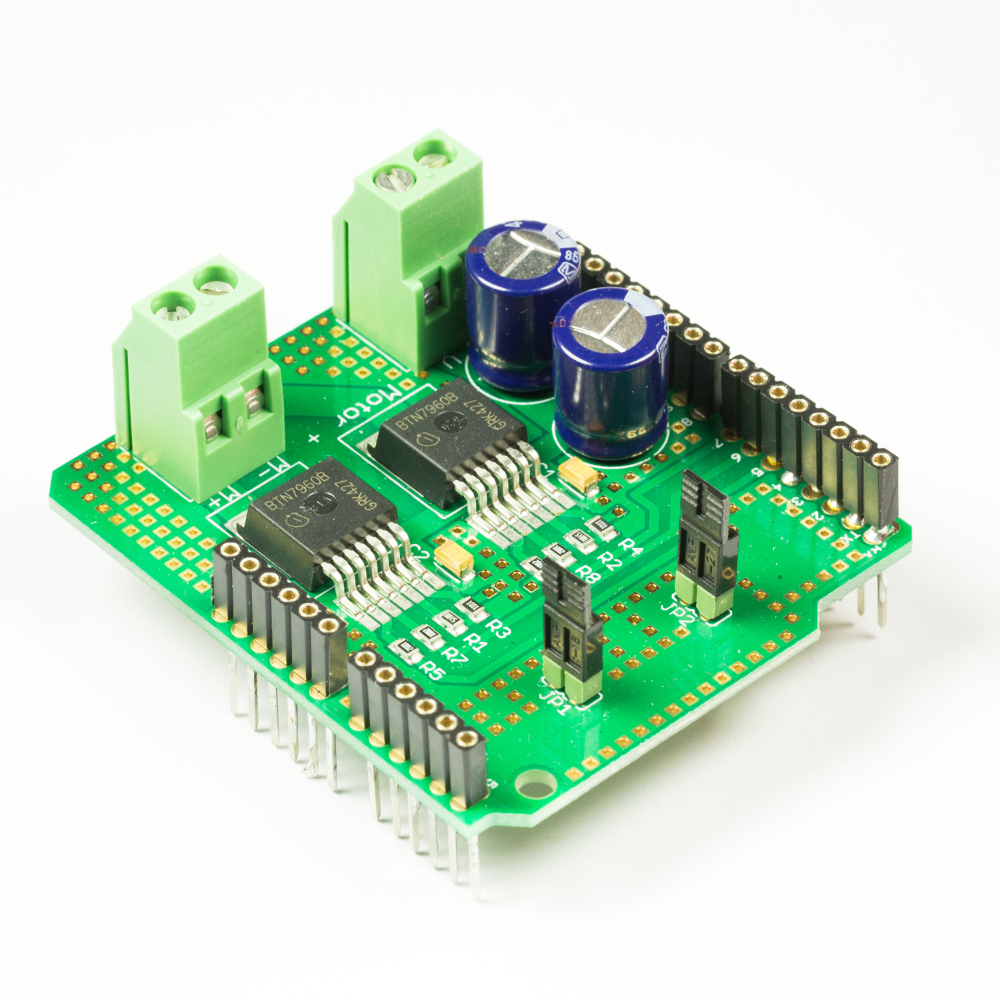
\includegraphics[width=0.4\textwidth]{./images/highpower-motorshield.jpg}
			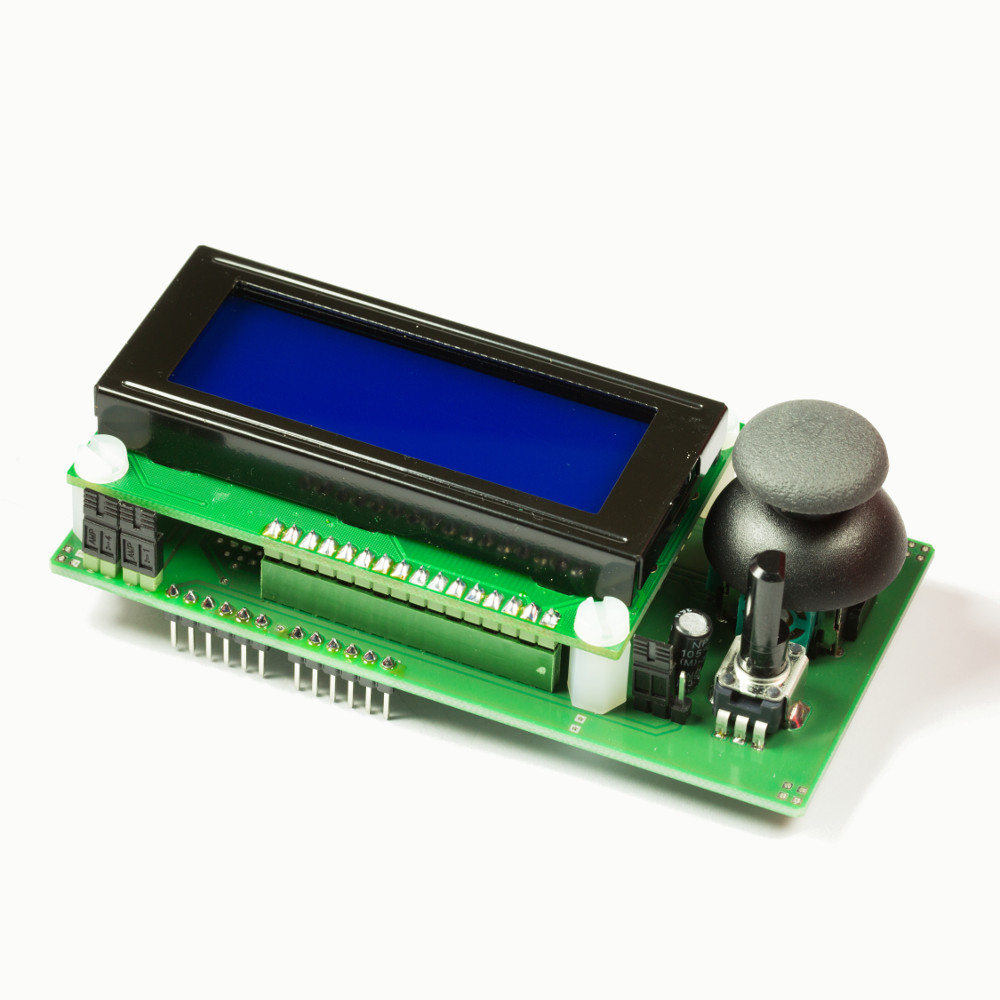
\includegraphics[width=0.4\textwidth]{./images/display-shield.jpg}\\
			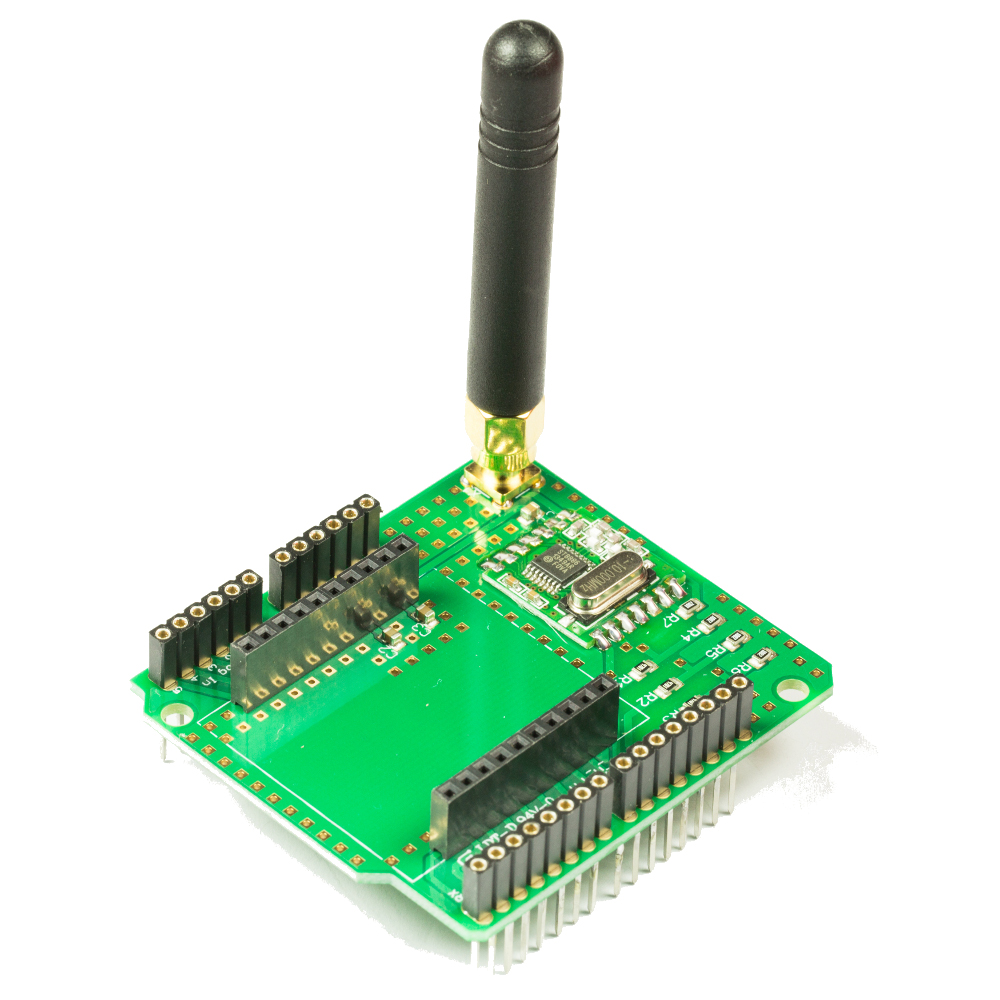
\includegraphics[width=0.4\textwidth]{./images/funk-shield.jpg}
			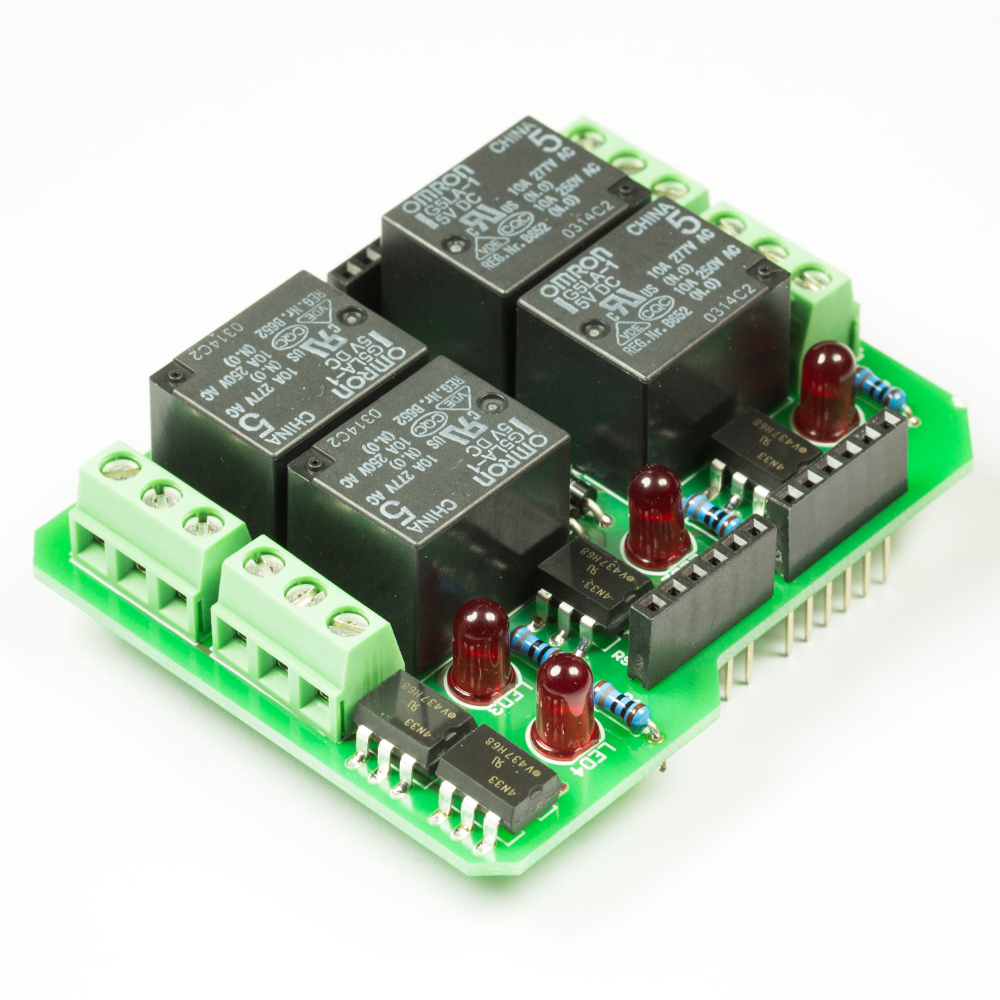
\includegraphics[width=0.4\textwidth]{./images/relais-shield.jpg}
		\end{figure}
	\end{column}
\end{columns}
\end{frame}
%%----------------------------------------------------------------------------------------
\begin{frame}[fragile]{Arduino Shields (2)}
\begin{itemize}
	\item \textbf{Open Source Arduino Libraries} erleichtern die direkte Verwendung von Arduino Shields 
\end{itemize}
\begin{itemize}
	\item \textbf{Komplexe Sachverhalte} (wie z.B. die Ansteuerung eines Gleichstrommotors \"uber Puls-Weiten-Modulation) \textbf{werden hinter einfach zu benutzenden Schnittstellen versteckt}
\end{itemize}
\begin{lstlisting}[frame=single, language=C]
static void        begin();

static void        set_speed(uint8_t const speed);
static uint8_t     get_speed();

static void        set_direction(E_DIRECTION const dir);
static E_DIRECTION get_direction();
\end{lstlisting}
\end{frame}
%%----------------------------------------------------------------------------------------
\begin{frame}{Wegbereiter der DIY-Revolution}
\begin{itemize}
	\item \textbf{2005}: 200 (Erstauflage)\cite{IEEE:2016:TheMakingOfArduino}
\end{itemize}
\begin{itemize}
	\item \textbf{2011}: $\approx$ 250 000\cite{IEEE:2016:TheMakingOfArduino}
\end{itemize}
\begin{itemize}
	\item \textbf{2013}: $\approx$ 700 000\cite{Quora:ArduinoSalesNumbers}
	\begin{itemize}
		\item + $\approx$ 700 000 Arduino Clones
	\end{itemize}
\end{itemize}
\vspace{10px}
\begin{itemize}
	\item Genaue Zahlen aufgrund der durch das Open-Hardware Konzept bedingten Arduino Clones schwer zu ermitteln
\end{itemize}
\end{frame}
%%----------------------------------------------------------------------------------------
\begin{frame}{Sergeant Pain}
 \begin{figure}[H]
  \centering
  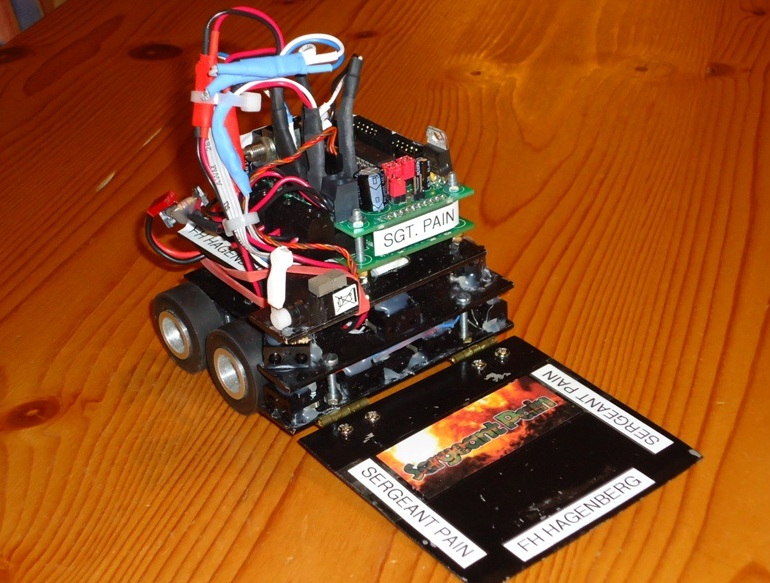
\includegraphics[width=0.7\textwidth]{./images/robot-sergeant-pain.jpg}
 \end{figure}
\end{frame}
%%----------------------------------------------------------------------------------------
\begin{frame}{\"Uberblick}
\begin{large}\textbf{Ziel}\end{large}
\begin{itemize}
	\item Autonome Erkennung des gegnerischen Roboters um diesen anschlie\ss{}end aus dem Ring zu schieben \href{./videos/sergeant-pain.mp4}{\beamergotobutton{Video}}
\end{itemize}
\vspace{20px}
\begin{large}\textbf{I/O}\end{large}
\begin{itemize}
	\item Sensoren
	\begin{itemize}
		\item 7 x Infrarotdistanzsensoren (Digitaler Eingang)
		\item 1 x Kippschalter (Digitaler Eingang)
	\end{itemize}
	\item Aktoren
	\begin{itemize}
		\item 2 x Gleichstromgetriebemotoren (Puls-Weiten-Modulation)
		\item 1 x RC Servo (Puls-Weiten-Modulation)
	\end{itemize}
\end{itemize}
\end{frame}
%%----------------------------------------------------------------------------------------
\begin{frame}{Umsetzung}
\begin{columns}
	\begin{column}{0.7\textwidth}
\begin{itemize}
	\item Entwicklung 2010/11 $\rightarrow$ Arduino zwar verf\"ugbar, aber noch nicht bekannt $\rightarrow$ \textbf{RN-MiniControl} + \textbf{RN-VN2DualMotor}
\end{itemize}
\begin{itemize}
	\item RN-MiniControl:
	\begin{itemize}
		\item ATMega168 als $\mu$C
		\item I/Os werden auf Stift/Buchsenleisten herausgef\"uhrt
		\item Einsteckbare Platinen (wie z.B RN-VN2DualMotor f\"ur die Motorsteuerung)
		\item Programmierung via \textbf{BASIC} oder \textbf{C (AVR Studio)}
	\end{itemize}
\end{itemize}
\begin{itemize}
	\item Konzept der \textbf{RN-MiniControl} weist \textbf{starke \"Ahnlichkeiten mit dem Arduino} Konzept auf, \textbf{ABER} nach wie vor \textbf{Kenntnisse der Embedded Programmierung notwendig}
\end{itemize}
	\end{column}
	\begin{column}{0.3\textwidth}
	\begin{figure}
		\centering
		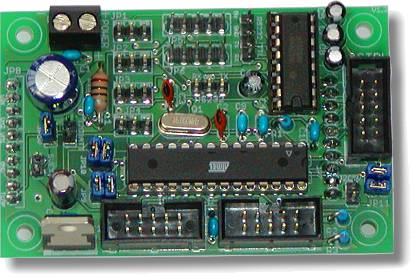
\includegraphics[width=0.8\textwidth]{./images/rn-minicontrol.jpg}
		\caption{RN-MiniControl\cite{Image:RNMiniControl}}
	\end{figure}
	\begin{figure}
		\centering
		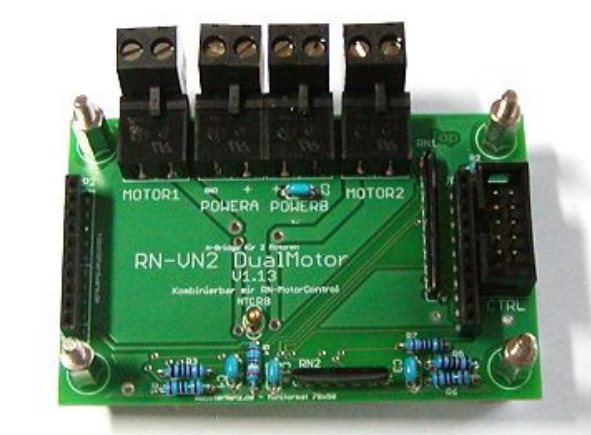
\includegraphics[width=0.8\textwidth]{./images/rn-vnh2dualmotor.jpg}
		\caption{RN-VN2Dual...\cite{Image:RNVN2DualMotor}}
	\end{figure}
	\end{column}
\end{columns}
\end{frame}
%%----------------------------------------------------------------------------------------
\begin{frame}{Evolution}
 \begin{figure}[H]
  \centering
  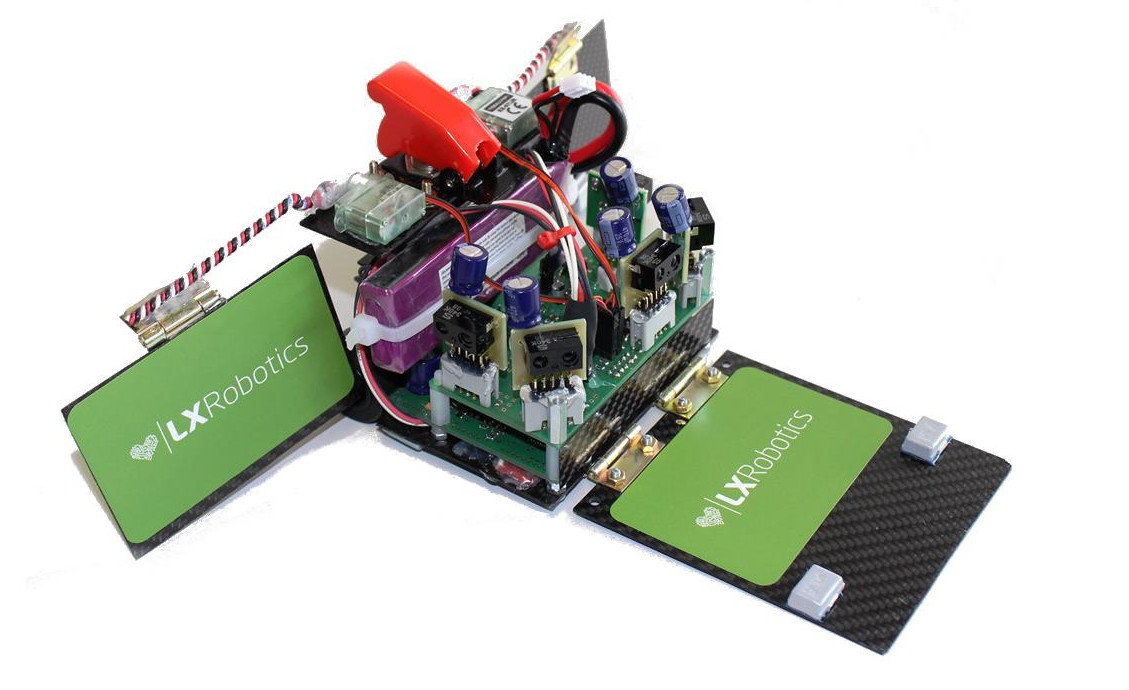
\includegraphics[width=0.7\textwidth]{./images/robot-evolution.jpg}
 \end{figure}
\end{frame}
%%----------------------------------------------------------------------------------------
\begin{frame}{\"Uberblick}
\begin{large}\textbf{Ziel}\end{large}
\begin{itemize}
	\item Autonome Erkennung des gegnerischen Roboters um diesen anschlie\ss{}end aus dem Ring zu schieben
\end{itemize}
\vspace{20px}
\begin{large}\textbf{I/O}\end{large}
\begin{itemize}
	\item Sensoren
	\begin{itemize}
		\item 5 x Infrarotdistanzsensoren (Digitaler Eingang)
		\item 1 x Infrarotstartmodul (Digitaler Eingang)
	\end{itemize}
	\item Aktoren
	\begin{itemize}
		\item 2 x Brushless Outrunner Motoren
		\item 2 x RC Servos (Puls-Weiten-Modulation)
	\end{itemize}
\end{itemize}
\end{frame}
%%----------------------------------------------------------------------------------------
\begin{frame}{Umsetzung (1)}
\begin{itemize}
	\item Dezidierter $\mu$C f\"ur die Ansteuerung eines Brushless Motors notwendig $\rightarrow$ 3 $\mu$Cs ben\"otigt
	\begin{itemize}
		\item \textbf{$\mu$C1/2}: Steuerung des linken/rechten Motors
		\item \textbf{$\mu$C3}: Auswertung der Sensoren und entsprechende Ansteuerung von $\mu$C1 und 2
	\end{itemize}
\end{itemize}
\begin{itemize}
	\item Entwicklung 2014 $\rightarrow$ Arduino Konzept bekannt, ABER \textbf{mechanische Abmessungen} von Arduino \textbf{verhindern optimale Ausn\"utzung} des vorhandenen Platzes
\end{itemize}
\begin{itemize}
	\item Ausgehend vom Shield Gedanken wird \"ahnlich Sergeant Pain ein \textbf{Motorboard und} ein \textbf{Brainboard} entwickelt
\end{itemize}
\end{frame}
%%----------------------------------------------------------------------------------------
\begin{frame}{Umsetzung (2)}
\begin{columns}
	\begin{column}{0.8\textwidth}
\begin{itemize}
	\item \textbf{Motorboard}:
	\begin{itemize}
		\item 2 x ATMega328 (Arduino Uno)
		\item 2 x 3 Halbbr\"ucken f\"ur Ansteuerung der Brushlessmotoren +
		\item 2 x BEMF Filternetzwerk (Elektronik \"ahnlich dem LXRobotics Brushless Motorshield)
	\end{itemize}
\end{itemize}
\begin{itemize}
	\item \textbf{Brainboard}:
	\begin{itemize}
		\item 1 x ATMega32U4 (Arduino Leonardo)
		\item Buchsenleisten f\"ur das Einstecken der Infrarotdistanzsensoren sowie des Infrarotstartmoduls
		\item Kommunikation mit Motorboard via I2C
	\end{itemize}
\end{itemize}
	\end{column}
	\begin{column}{0.2\textwidth}
		\begin{figure}
			\centering
			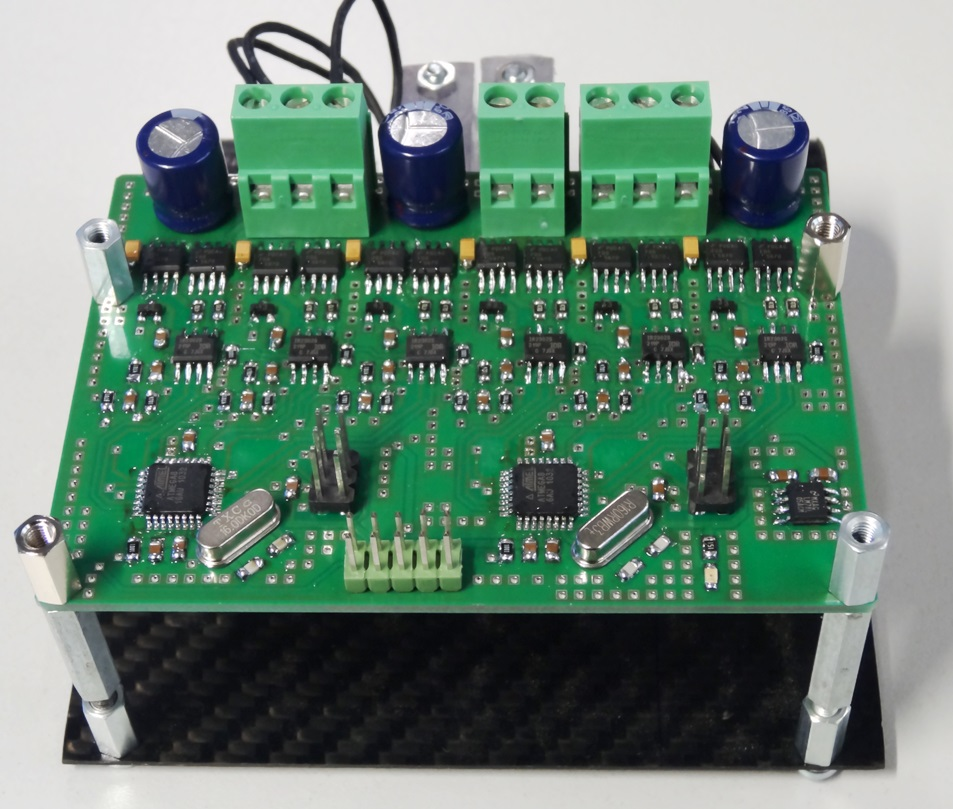
\includegraphics[width=1.0\textwidth]{./images/evolution-motorboard.jpg}
			\caption{Evolution Motorboard}
		\end{figure}
	\end{column}
\end{columns}
\vspace{20px}
\begin{itemize}
	\item \textbf{Implementierung der Softare} f\"ur sowohl Motorboard als auch Brainboard \textbf{als Arduino Libraries}
\end{itemize}
\end{frame}
%%----------------------------------------------------------------------------------------
\begin{frame}{Schnauzer}
 \begin{figure}[H]
  \centering
  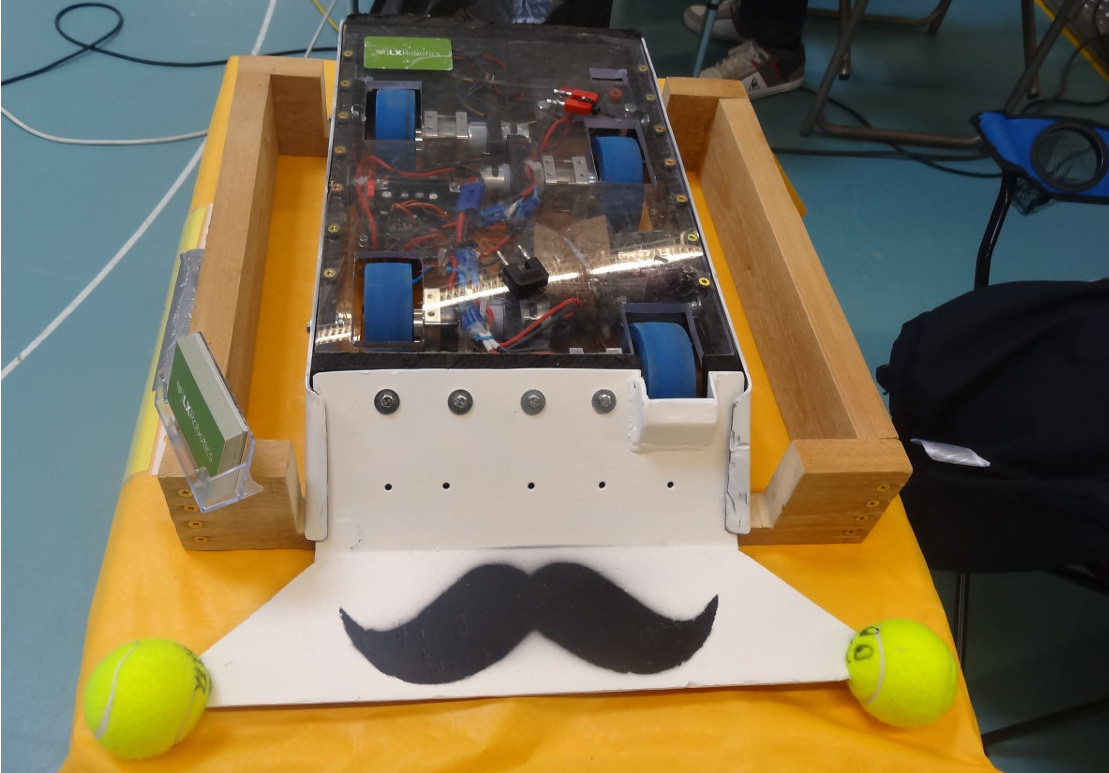
\includegraphics[width=0.7\textwidth]{./images/robot-schnauzer.jpg}
 \end{figure}
\end{frame}
%%----------------------------------------------------------------------------------------
\begin{frame}{\"Uberblick}
\begin{large}\textbf{Ziel}\end{large}
\begin{itemize}
	\item Den oder die gegnerischen Schaukampfroboter fahrunf\"ahig machen oder in die Arenagrube versenken.
\end{itemize}
\vspace{20px}
\begin{large}\textbf{Schaukampfroboter $\neq$ Roboter}\end{large}
\begin{itemize}
	\item Das \textbf{Sense - Think - Act} Paradigma wird nicht erf\"ullt
	\item "Nur" leistungsf\"ahiges ferngesteuertes Funktionsmodell
\end{itemize}
\vspace{20px}
\begin{large}\textbf{Wie passt Arduino ins Konzept?}\end{large}
\end{frame}
%%----------------------------------------------------------------------------------------
\begin{frame}{Arduino als elektronischer Fahrtregler (ESC) (1)}
\begin{itemize}
	\item Arduino wird als \textbf{ESC} eingesetzt
	\begin{itemize}
		\item Arduino setzt \textbf{Signale des Fernsteuerungsempf\"angers} auf \textbf{Motorsteuerkommandos} f\"ur \textbf{Motorshield} um
	\end{itemize}
\end{itemize}
 \begin{figure}[H]
 	\centering
 	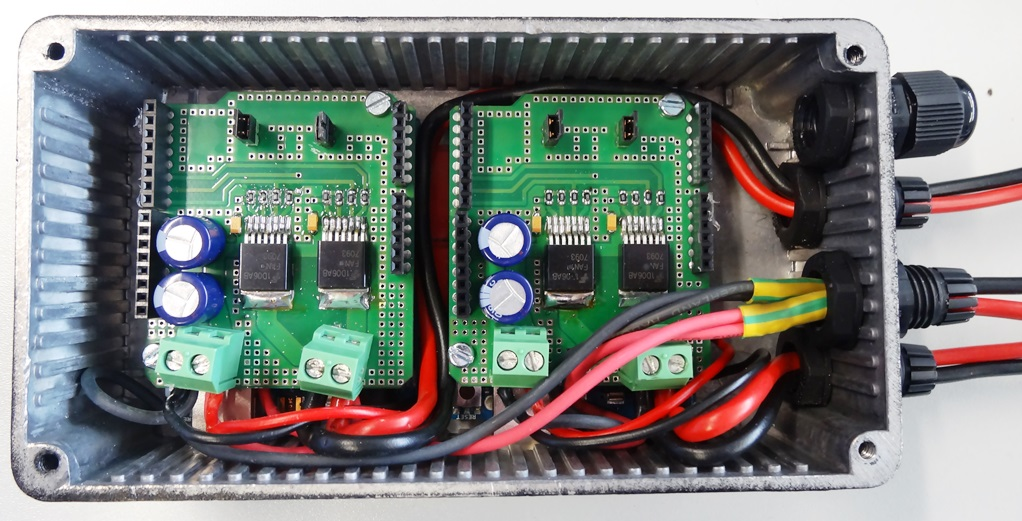
\includegraphics[width=0.7\textwidth]{./images/arduino-schnauzer.jpg}
 \end{figure}
\end{frame}
%%----------------------------------------------------------------------------------------
\begin{frame}{Arduino als elektronischer Fahrtregler (ESC) (2)}
\begin{itemize}
	\item \textbf{Steroid}: Entwicklung einer eigenen Arduino basierten ESC Platine
	\begin{itemize}
		\item Vermeidung von Kabelbruch als Fehlerquelle
		\item Kleinere Abmessungen m\"oglich
	\end{itemize}
\end{itemize}
\begin{figure}[H]
 	\centering
 	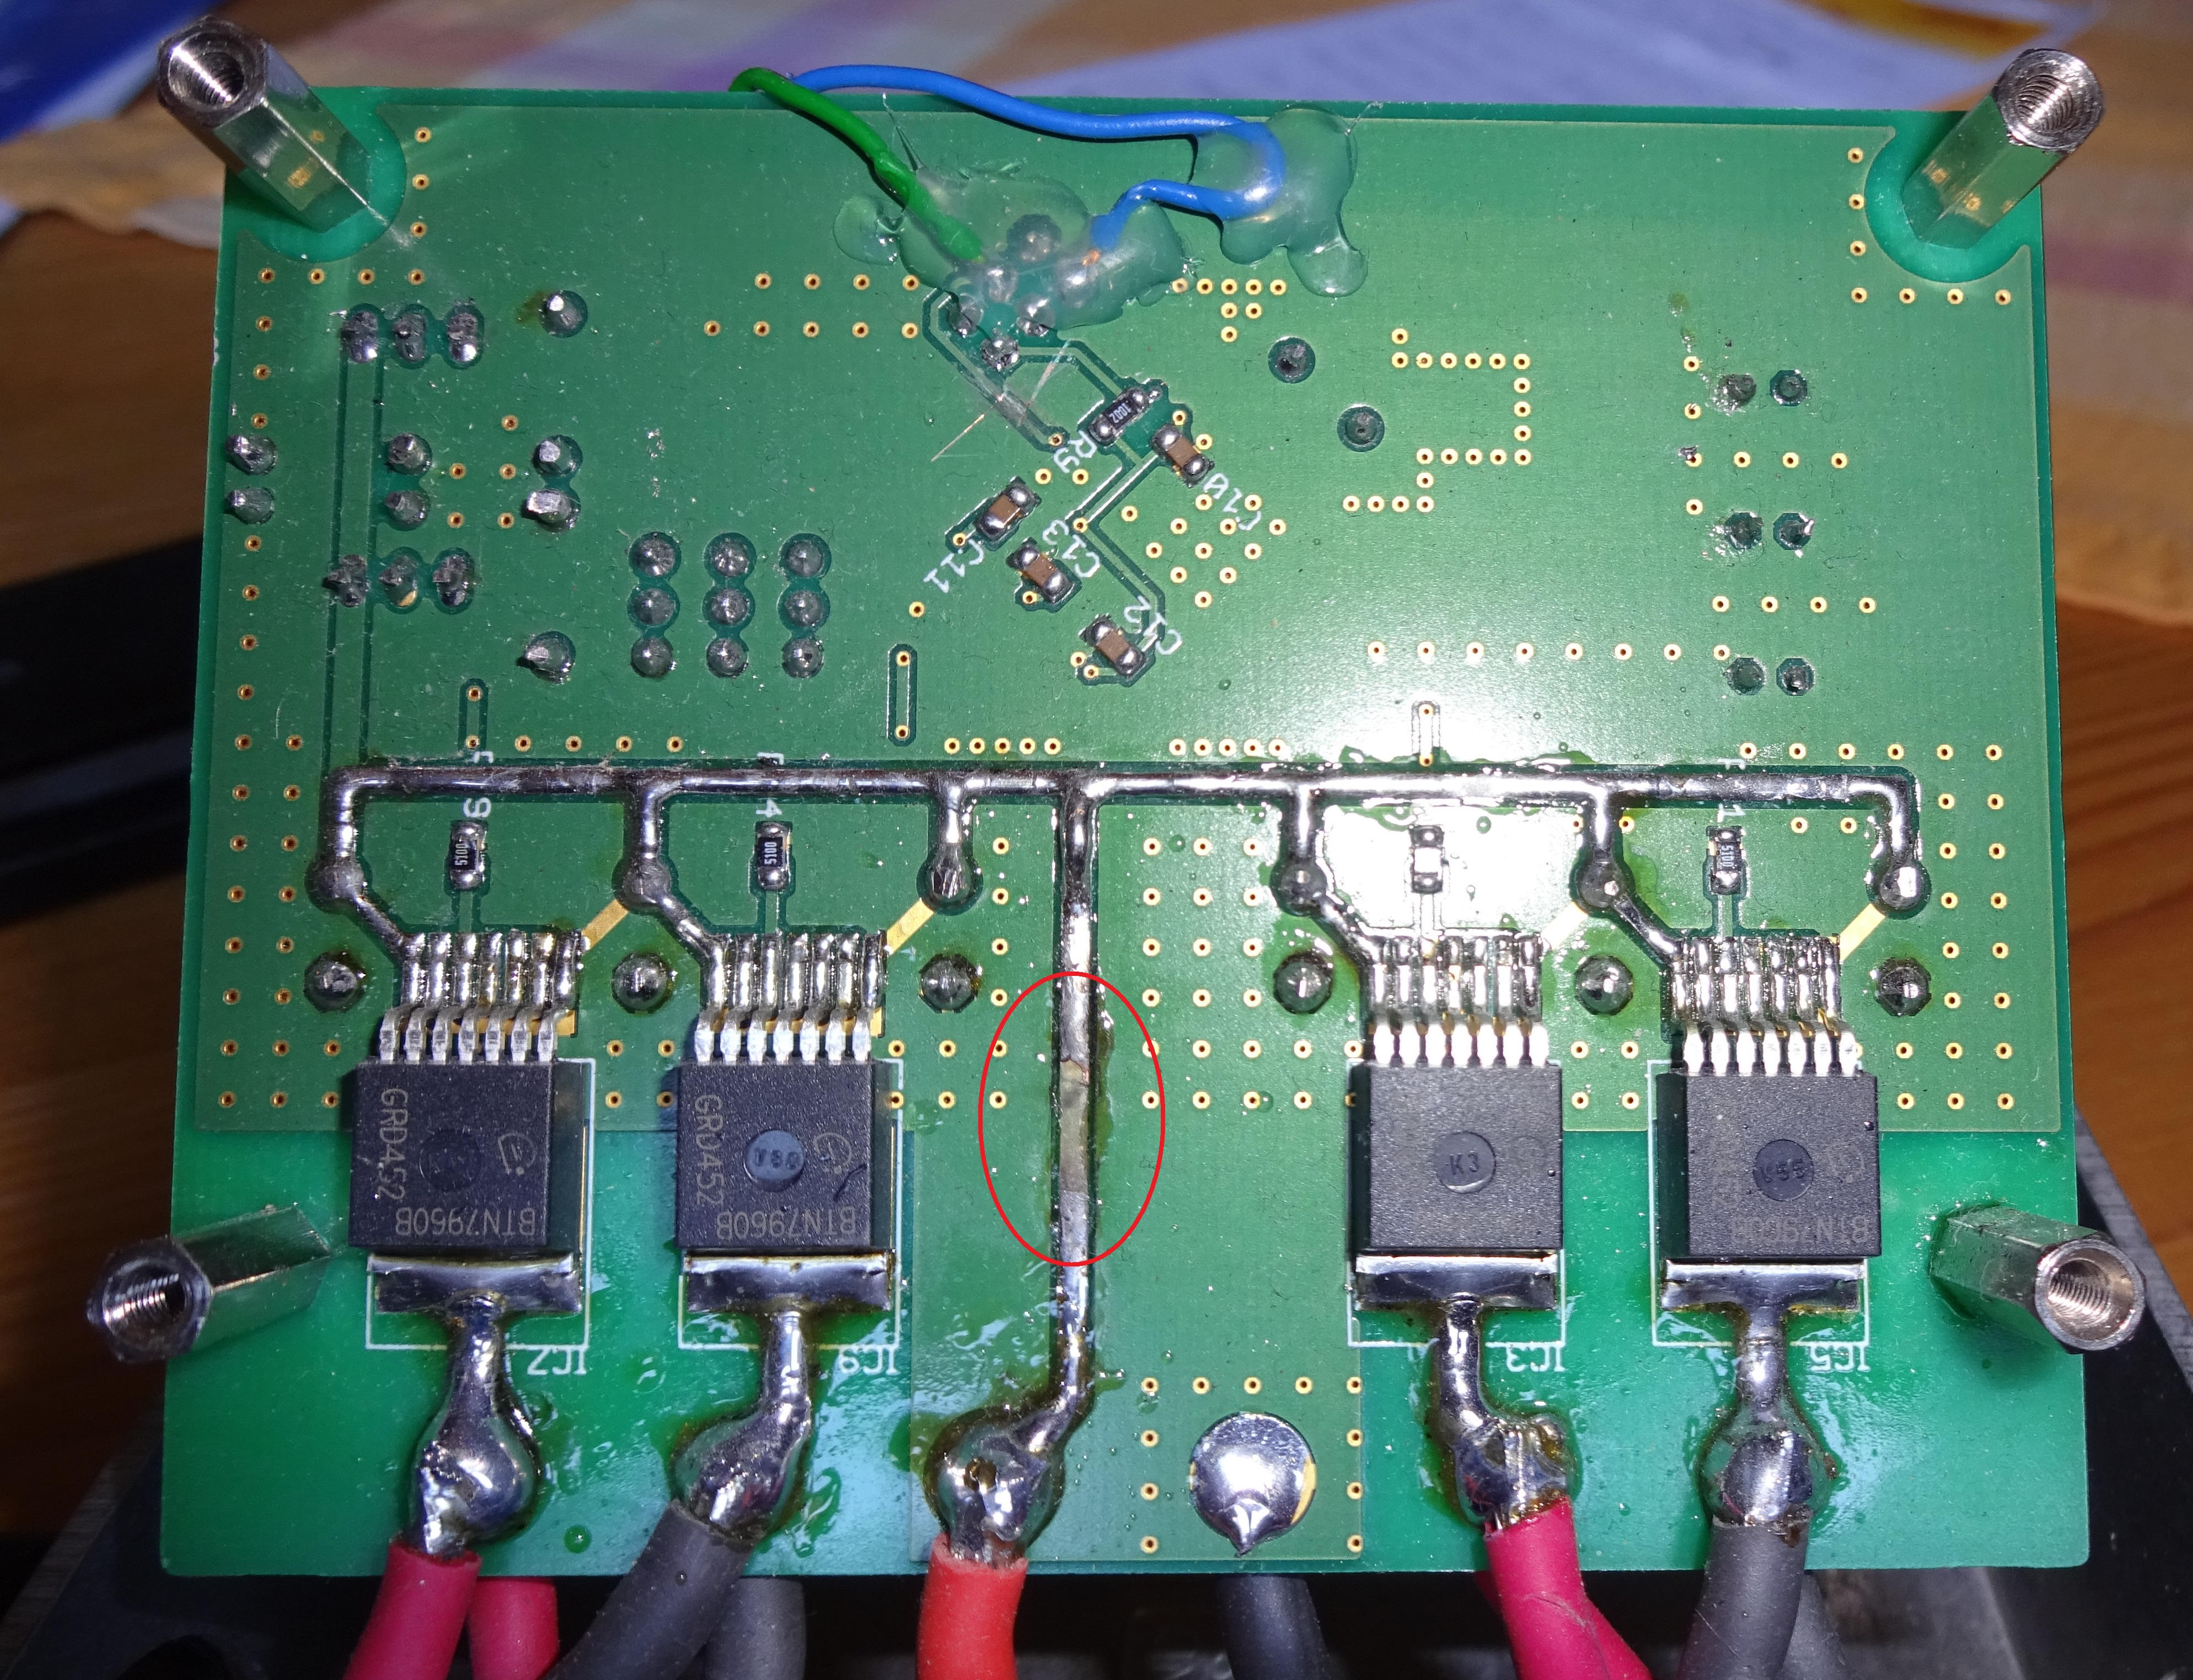
\includegraphics[width=0.6\textwidth]{./images/arduino-steroid.jpg}
\end{figure}
\end{frame}
%%----------------------------------------------------------------------------------------
\begin{frame}{Beauty Queen}
 \begin{figure}[H]
  \centering
  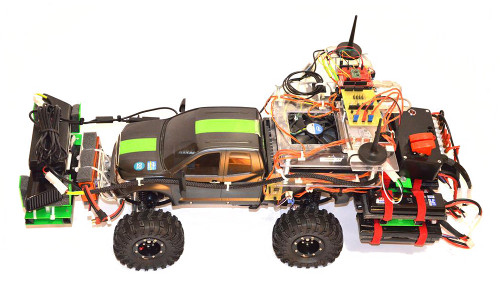
\includegraphics[width=0.7\textwidth]{./images/robot-beauty-queen.jpg}
 \end{figure}
\end{frame}
%%----------------------------------------------------------------------------------------
\begin{frame}{\"Uberblick (1)}
\begin{large}\textbf{Ziel}\end{large}
\begin{itemize}
	\item Umbau eines konventionellen RC-Automodellbausatzes in ein Fahrzeug f\"ur Simultaneous Localization and Mapping
\end{itemize}
\vspace{20px}
\begin{large}\textbf{I/O}\end{large}
\begin{itemize}
	\item Sensoren
	\begin{itemize}
		\item 1 x Microsoft Kinect
		\item 1 x IMU
		\item 2 x Reifenumdrehungssensoren
	\end{itemize}
	\item Aktoren
	\begin{itemize}
		\item 1 x Getriebeservo (Puls-Weiten-Modulation)
		\item 1 x Lenkservo (Puls-Weiten-Modulation)
		\item 1 x Electronic Speed Controller (Puls-Weiten-Modulation)
	\end{itemize}
\end{itemize}	
\end{frame}
%%----------------------------------------------------------------------------------------
\begin{frame}{\"Uberblick (2)}
\begin{itemize}
	\item \textbf{Problem}
	\begin{itemize}
		\item Sensordaten k\"onnen nicht durch ein Arduino ausgewertet werden $\rightarrow$ vollst\"andiger PC notwendig
		\item PC kann wiederum nicht direkt mit Sensoren/Aktoren kommunizieren
	\end{itemize}
\end{itemize}
\begin{itemize}
	\item \textbf{L\"osung}: Entwicklung eines Arduino-I/O-Systems als Vermittler zwischen den Sensoren/Aktoren und dem PC
\end{itemize}
\end{frame}
%%----------------------------------------------------------------------------------------
\begin{frame}{Arduino-I/O-System: Motivation}
	\begin{itemize}
		\item Die Entwicklung von autonomen Systemen erfordert einen \textbf{enormen Zeitaufwand}
		\begin{itemize}
			\item \textbf{Hardware}, \textbf{Soft}- und \textbf{Firmware}
			\item \textbf{Schnittstellen} und \textbf{Kommunikationsprotokolle} zwischen den zahlreichen Subsystemen
		\end{itemize}
	\end{itemize}
	\begin{itemize}
		\item \textbf{Beobachtung}: Viele Sensoren und Aktoren haben identische Schnittstellen
		\begin{itemize}
			\item IR Distanzsensor/Temperatursensor/Lichtsensor  $\rightarrow$ Analoge Spannung
			\item Ultraschall Distanzsensor/Beschleunigungssensor/Gyroskop $\rightarrow$ I2C
			\item DC Motor, RC Servo Motor $\rightarrow$ Puls-Weiten-Modulation
		\end{itemize}
	\end{itemize}
	\begin{itemize}
		\item \textbf{Ziel}: Entwicklung eines I/O-Systems welche die meist verwendeten I/O-Funktionen in \textbf{einem wiederverwendbaren I/O-Modul} integriert
		\begin{itemize}
			\item \textbf{Reduzierung} der f\"ur die Entwicklung eines autonomen Systems ben\"otigte Zeit $\rightarrow$ Das Rad muss nicht immer wieder neu erfunden werden.
		\end{itemize}
	\end{itemize}
\end{frame}
%%----------------------------------------------------------------------------------------
\begin{frame}[fragile]{Arduino-I/O-System: Implementierung}
	\begin{itemize}
		\item \textbf{Hardware} (Arduino Uno) + \textbf{Software}
		\begin{itemize}
			\item Firmware f\"ur Arduino Uno
			\item C++ Library \textbf{libarduinoio}
		\end{itemize}
		\begin{figure}[htbp]
			\centering
			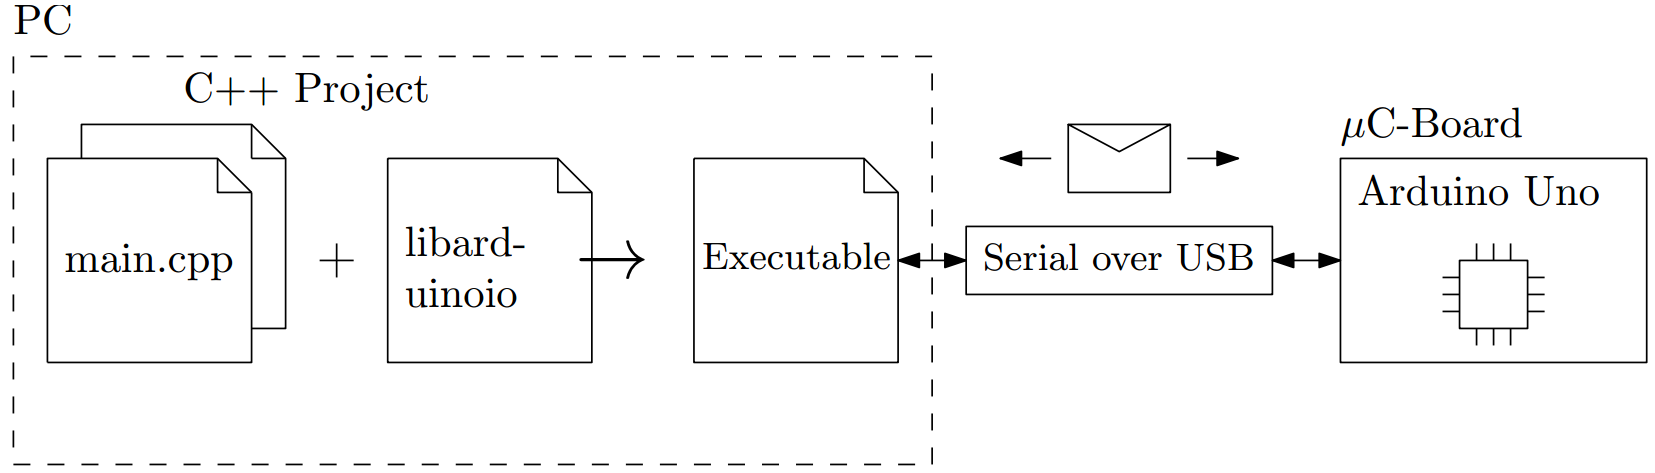
\includegraphics[scale=0.2]{./images/arduinoio-system-overview.png}
		\end{figure}
		\item \textbf{Highlevel Ansteuerung} von $\mu{}C$-I/O-Funktionen
	\end{itemize}
\begin{lstlisting}[frame=single, language=C]
auto oD2 = io.createGpioOutputPin(arduinoio::D2, false);
bool const success = oD2->setPinValue(true));
bool const pin_value = oD2->getPinValue();
\end{lstlisting}
\end{frame}
%%----------------------------------------------------------------------------------------
\begin{frame}{Arduino-I/O-System: Angebotene I/O-Funktionen}
	\begin{itemize}
		\item I/O-Funktion verf\"ugbar via $\mu{}C$-I/O-Pin:
		\begin{table}[htbp]
			\begin{tabular}{|c|c|}
				\hline 
				\textbf{I/O-Funktion} & \textbf{Anzahl von I/O-Einheiten} \\ 
				\hline \hline 
				Analoger Eingang & Max. 6 \\ 
				\hline 
				Digitaler Eingang & max. 12  \\ 
				\hline
				Digitaler Ausgang & max. 12 \\ 
				\hline
				Hardware PWM & max. 2 \\ 
				\hline
				Software PWM & max. 6 \\ 
				\hline
				Event Z\"ahler & max. 2 \\
				\hline
				I2C Br\"ucke & max. 1 \\
				\hline
			\end{tabular}
		\end{table}
		\item Weiters:
		\begin{itemize}
			\item Hardware-Reset
			\item 16-Bit Board-ID
			\item Chip-Temperature
		\end{itemize}
	\end{itemize}
\end{frame}
%%----------------------------------------------------------------------------------------
\begin{frame}{Arduino-I/O-System: Verifikation (1)}
	\begin{itemize}
		\item Die Verifikation der individuellen Komponenten ist nicht zielf\"uhrend $\rightarrow$ Verifikation des Gesamtsystems notwendig
	\end{itemize}
	\begin{itemize}
		\item Gesamtsystem = C++ Library, Kommunikationsschnittstelle, Arduino Firmware $\rightarrow$ \textbf{Ende-Zu-Ende-Verifikation}
	\end{itemize}
	\begin{itemize}
		\item \textbf{Idee}: Einige Pins werden als Eing\"ange, andere als Ausg\"ange definiert und diese auf \textbf{intelligente Art und Weise} miteinander verbunden
	\end{itemize}
	\begin{itemize}
		\item \textbf{Unit Test Framework} f\"ur automatische Ausf\"uhrung aller Tests
	\end{itemize}
\end{frame}
%%----------------------------------------------------------------------------------------
\begin{frame}{Arduino-I/O-System: Verifikation (2)}
	\begin{itemize}
		\item Digitale Ausg\"ange \textbf{erzeugen} analoge Spannungen via \textbf{R2R Widerstandsnetzwerk}
		\item Analoge Eing\"ange \textbf{messen} diese analogen Spannungen
		\item Testframework \textbf{vergleicht} die gemessene Spannung mit der berechneten Spannung
	\end{itemize}
	\begin{itemize}
		\item 12 digitale Ausg\"ange + 6 analoge Eing\"ange $\rightarrow$ \textbf{6 R2R Widerstandsnetzwerke} mit 2 Bit Aufl\"osung
	\end{itemize}
	\begin{columns}
		\begin{column}{0.4\textwidth}
			\begin{figure}[htbp]
				\centering
				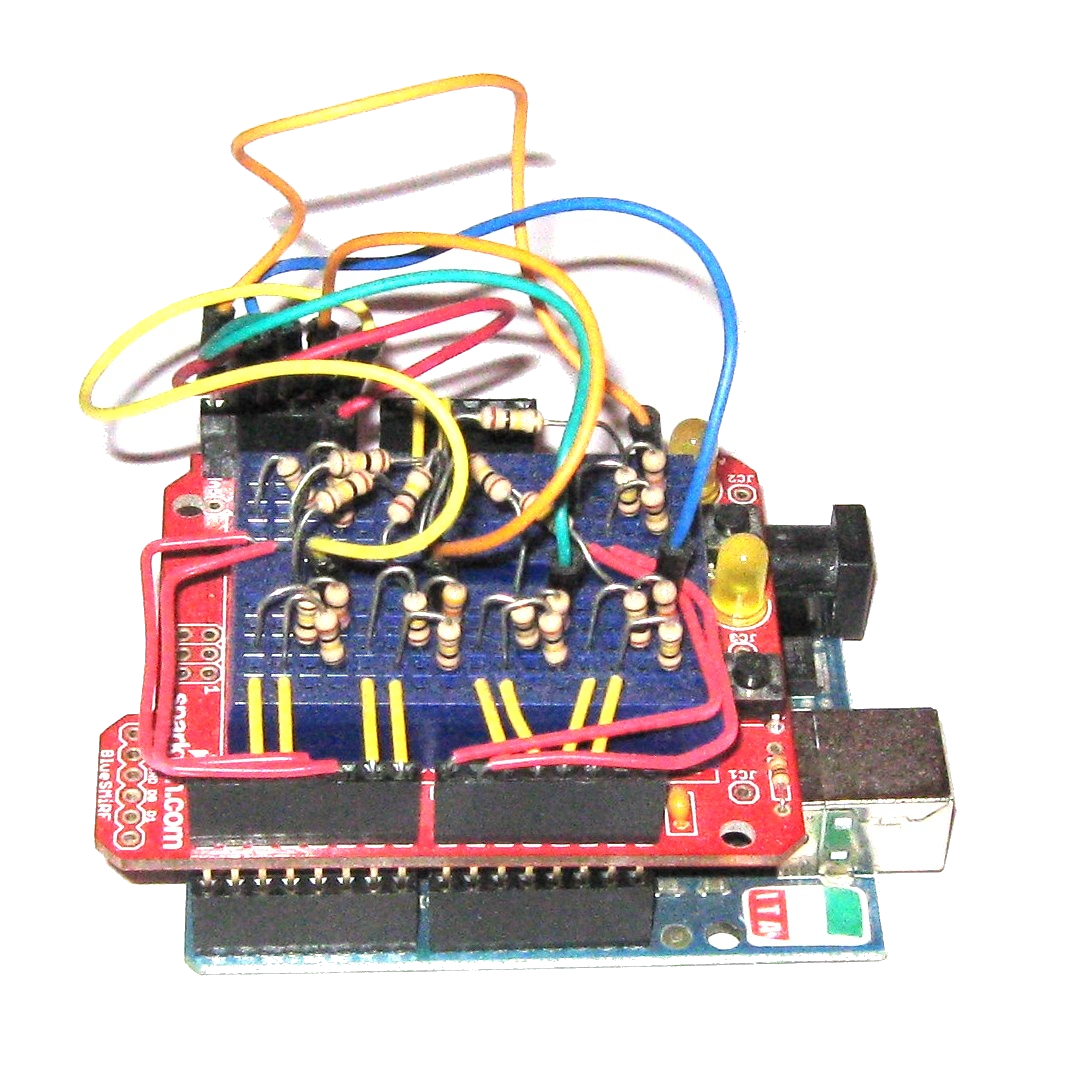
\includegraphics[scale=0.2]{./images/arduinoio-r2r.png}
			\end{figure}
		\end{column}
		\begin{column}{0.4\textwidth}
			\begin{figure}[htbp]
				\centering
				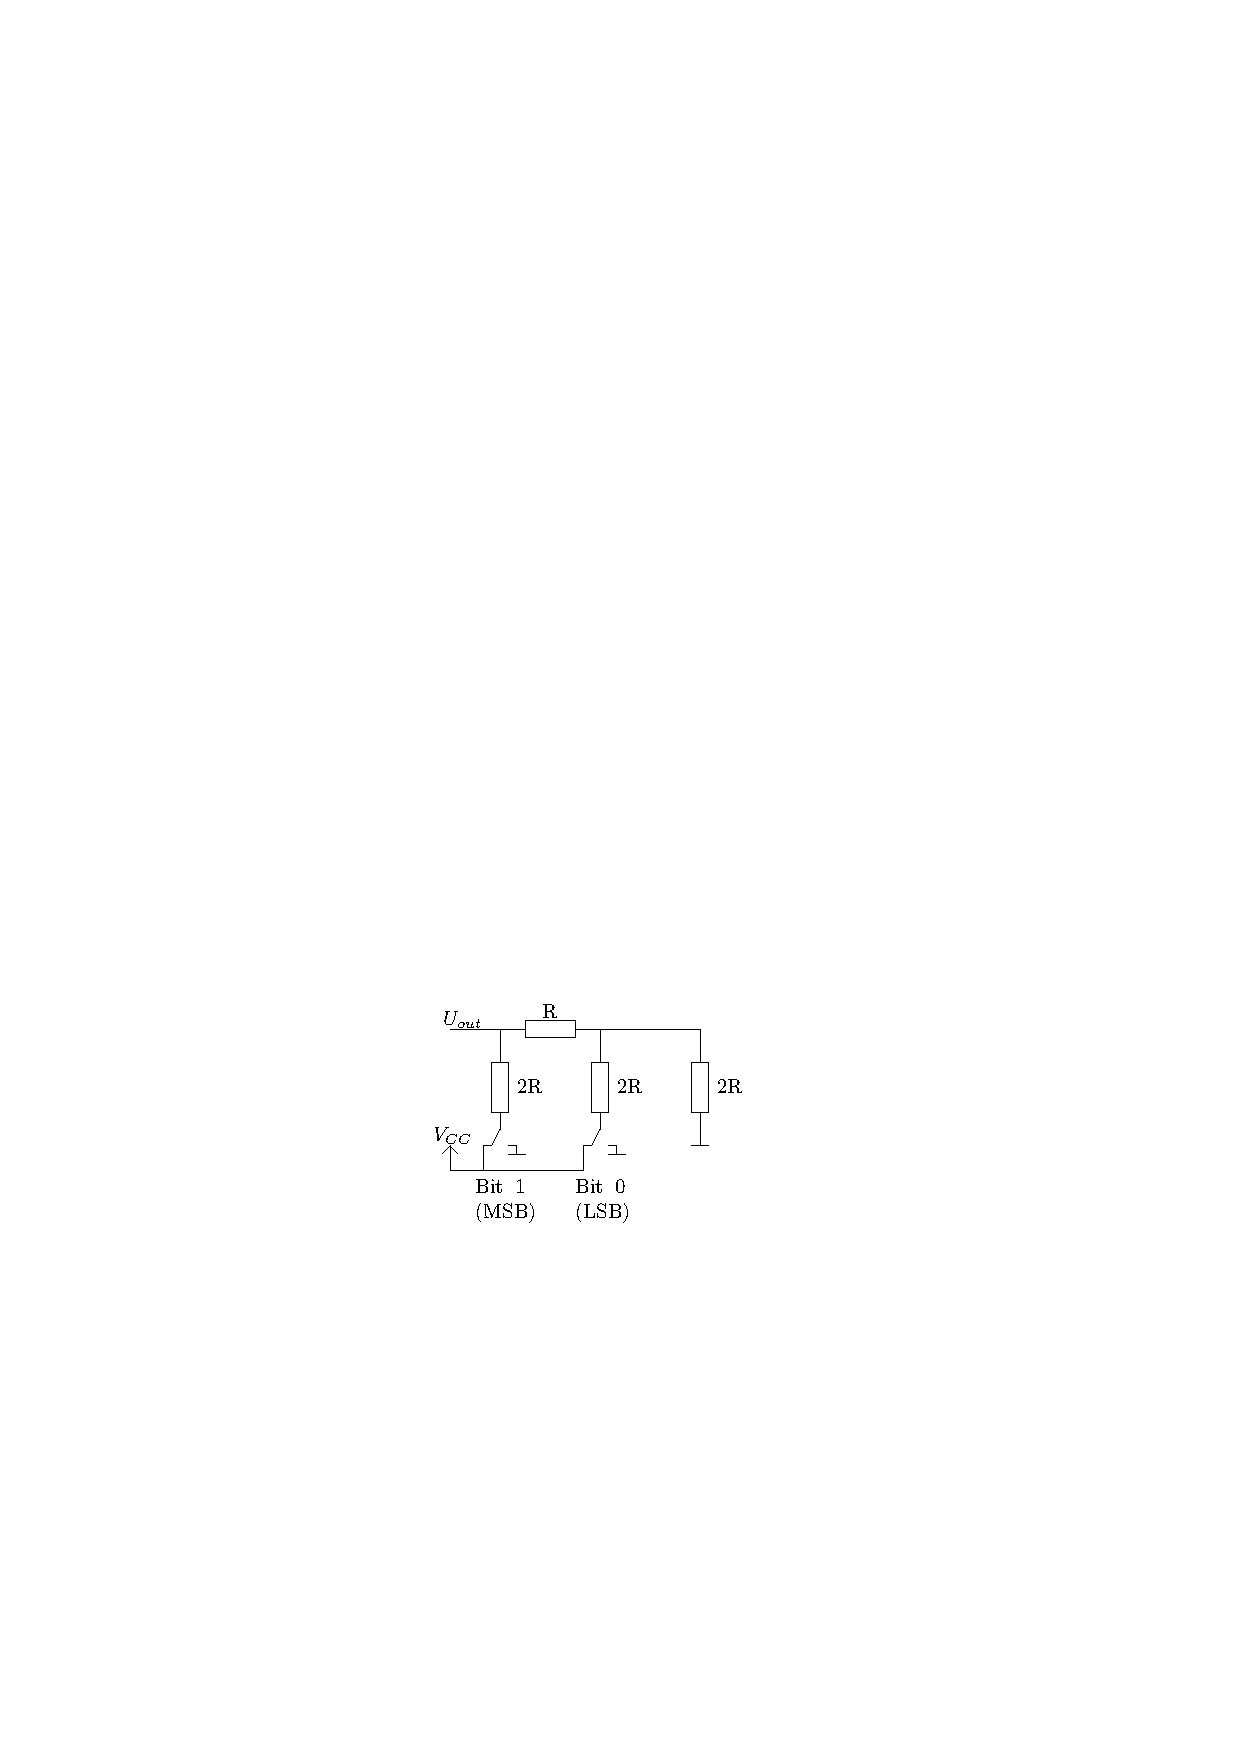
\includegraphics[scale=0.6]{./images/arduinoio-r2r-network.pdf}
			\end{figure}
		\end{column}
	\end{columns}
\end{frame}
%%----------------------------------------------------------------------------------------
\begin{frame}{Arduino-I/O-System: Timing}
	\begin{itemize}
		\item \textbf{Command execution time} (CED): Wie lange dauert ein I/O-Befehl?
	\end{itemize}
	\begin{table}[htbp]
		\begin{tabular}{|c|c|}
			\hline 
			\textbf{Command} & \textbf{CED, [CED] = ms} \\ 
			\hline \hline 
			Get ID & 4.15532 ms \\ 
			\hline 
			Set pin value & 4.64086 ms  \\ 
			\hline
			Get pin value & 4.6447 ms \\ 
			\hline
			Get analog value & 5.00152 ms \\ 
			\hline
			I2C Write (1 Byte)  & 4.88282 ms\\ 
			\hline
			I2C Read (1 Byte) & 6.25022 ms \\
			\hline
		\end{tabular}
	\end{table}
	\begin{itemize}
		\item \textbf{Schlussfolgerung}: Hauptanwendungsgebiet sind Applikationen bei denen die CED keine gro\ss{}e Rolle spielt, wie z.B.
		\begin{itemize}
			\item Steuerung von Status LEDs, \"Uberwachen der Batteriespannung, (RC Servo Ansteuerung), etc.
		\end{itemize}
	\end{itemize}
\end{frame}
%%----------------------------------------------------------------------------------------
\begin{frame}{Arduino-I/O-System: Anwendung in Beauty Queen}
\begin{large}\textbf{Aufgaben des Arduino-I/O-Systems:}\end{large}
 \begin{itemize}
  \item \textbf{Steuern}
  \begin{itemize}
   \item Electronic Speed Controller
   \item Lenk- und Getriebeservo
   \item Status LEDs
  \end{itemize}
 \end{itemize}
 \begin{itemize}
  \item \textbf{\"Uberwachen}
  \begin{itemize}
   \item Batteriespannung
  \end{itemize}
 \end{itemize}
\begin{large}\textbf{Einschr\"ankungen:}\end{large}
\begin{itemize}
 \item Arduino-I/O-System f\"ur Echtzeitanwendungen gar nicht/nur eingeschr\"ankt einsetzbar: Folgende I/O Funktionen wurden \"uber eine separate Firmware f\"ur den Bordrechner zur Verf\"ugung gestellt:
 \begin{itemize}
  \item Abfrage der Daten der IMU (Inertial Measurement Unit)
  \item Auswertung der Reifenencoder
 \end{itemize}
\end{itemize}
\end{frame}
%----------------------------------------------------------------------------------------
\begin{frame}{Arduino-I/O-System: Ressourcen}
	\begin{itemize}
		\item Der Quellcodes des Arduino-I/O-Systems steht unter der \textbf{BSD-3}-Lizenz
		\begin{itemize}
			\item Kann f\"ur kommerzielle Applikationen genutzt werden
		\end{itemize}
	\end{itemize}
	\begin{itemize}
		\item \url{https://github.com/lxrobotics/arduinoio}
	\end{itemize}
\end{frame}
%%----------------------------------------------------------------------------------------
\begin{frame}{Lex}
 \begin{figure}[H]
  \centering
  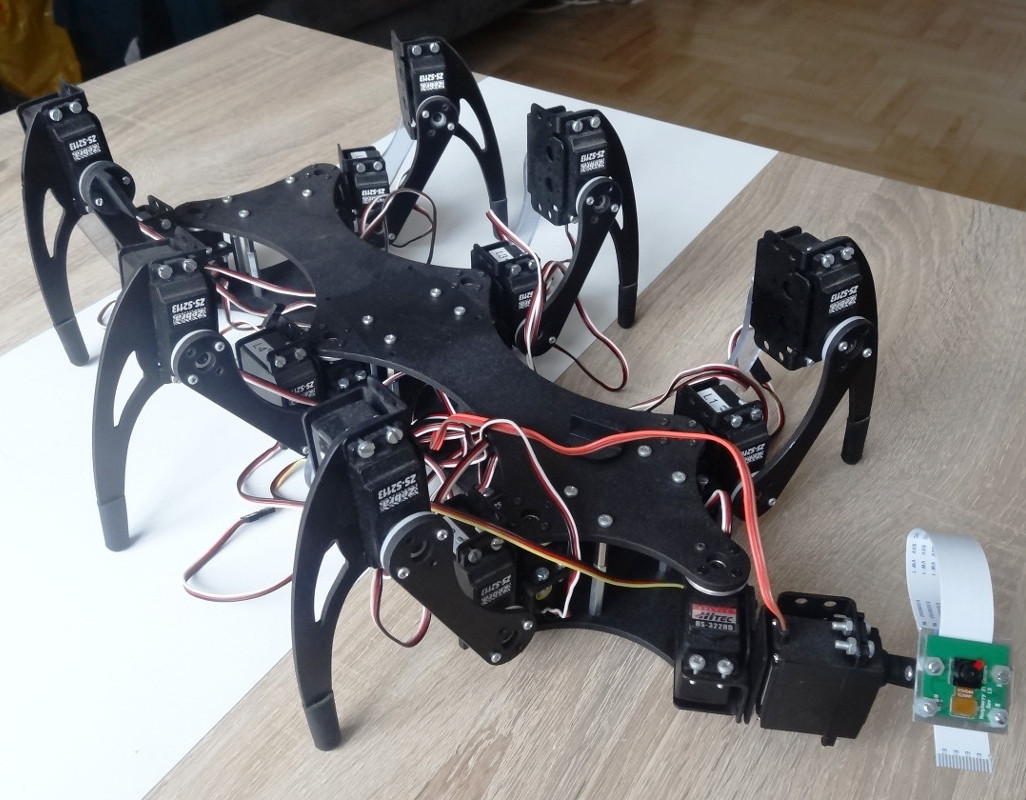
\includegraphics[width=0.7\textwidth]{./images/robot-lex.jpg}
 \end{figure}
\end{frame}
%%----------------------------------------------------------------------------------------
\begin{frame}{\"Uberblick}
\begin{large}\textbf{Ziel}\end{large}
\begin{itemize}
	\item Bau eines Hexapods (weil es Spa\ss{} macht \Smiley{})
\end{itemize}
\vspace{20px}
\begin{large}\textbf{I/O}\end{large}
\begin{itemize}
	\item Sensoren
	\begin{itemize}
		\item RaspberryPiCam
	\end{itemize}
	\item Aktoren
	\begin{itemize}
		\item 6 x 3 RC Servos (Beine) (Puls-Weiten-Modulation)
		\item 2 RC Servos (Kopf) (Puls-Weiten-Modulation)
	\end{itemize}
\end{itemize}
\end{frame}
%%----------------------------------------------------------------------------------------
\begin{frame}{Umsetzung}
\begin{itemize}
	\item \textbf{Erster Ansatz}: Servo Shield + Ansteuerung via I2C-Br\"ucke des Arduino-I/O-Systems
\end{itemize}
\begin{itemize}
	\item \textbf{Problem}: Arduino-I/O-System nicht schnell genug f\"ur Kommunikation der ben\"otigten Steuersignale an das Servo Shield
\end{itemize}
\begin{itemize}
	\item \textbf{Neuer Ansatz} unter Einbeziehung des \textbf{Robot Operating System} (ROS)
\end{itemize}
\end{frame}
%----------------------------------------------------------------------------------------
\begin{frame}{Was ist ROS?}
\begin{alertblock}{ROS}
\textit{The Robot Operating System (ROS) is a flexible framework for writing robot software. It is a collection of tools, libraries and conventions that aim to simplify the task of creating complex and robust robot behavior across a wide variety of robotic platforms.}
\end{alertblock}
\end{frame}
%%----------------------------------------------------------------------------------------
\begin{frame}{ROS Basics: Node}
\begin{alertblock}{Node ...}
... bezeichnet einen Prozess, der Berechnungen ausf\"uhrt.
\end{alertblock}
\begin{itemize}
	\item Typische Applikation besteht aus mehreren Nodes
	\item Die Bezeichnung \textbf{Node} stammt von der graphischen Abbildung aller laufenden Prozesse sowie der Kommunikation zwischen den Prozessen als \textbf{gerichteter Graph} (Tool: \textbf{rqt\_graph})
	\item Eindeutige Identifikation eines Prozesses durch einen \textbf{Graph Ressource Name} (''Nodename'')
\end{itemize}
\begin{figure}[H]
	\centering
	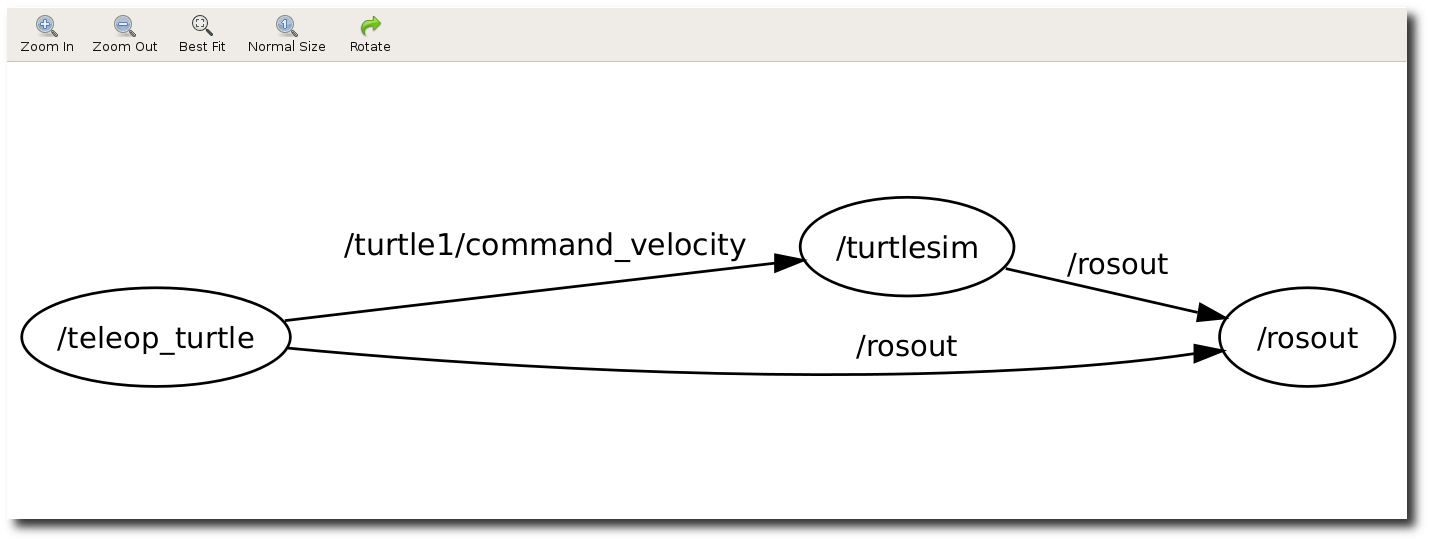
\includegraphics[width=0.6\textwidth]{./images/rxgraph-turtle-key.png}
	\caption{Source: \cite{ROS:2015:Online}}
	\label{fig:ros_graph}
\end{figure}
\end{frame}
%%----------------------------------------------------------------------------------------
\begin{frame}{ROS Basics: Message}
\begin{alertblock}{Messages ...}
... werden zur Kommunikation zwischen Nodes eingesetzt und sind eine Datenstruktur, welche aus typisierten Eintr\"agen besteht.
\end{alertblock}
\end{frame}
%%----------------------------------------------------------------------------------------
\begin{frame}{ROS Basics: Topic}
\begin{alertblock}{Topic ...}
... bezeichnet einen eindeutigen Namen den die Nodes zum Auffinden ihrer Kommunikationspartner f\"ur den Austausch von Messages ben\"otigen.
\end{alertblock}
\begin{itemize}
	\item Erzeugung und Verbrauch von Daten ist \textbf{entkoppelt} (Producer/Consumer-Pattern)
	\begin{itemize}
		\item Datenquellen/Source (\textbf{publish/ver\"offentlichen}) Messages zu einem Topic
		\item Datensenken/Sink (\textbf{subscribe/abbonieren}) Messages von einem Topic
	\end{itemize}
	\begin{figure}[H]
		\centering
		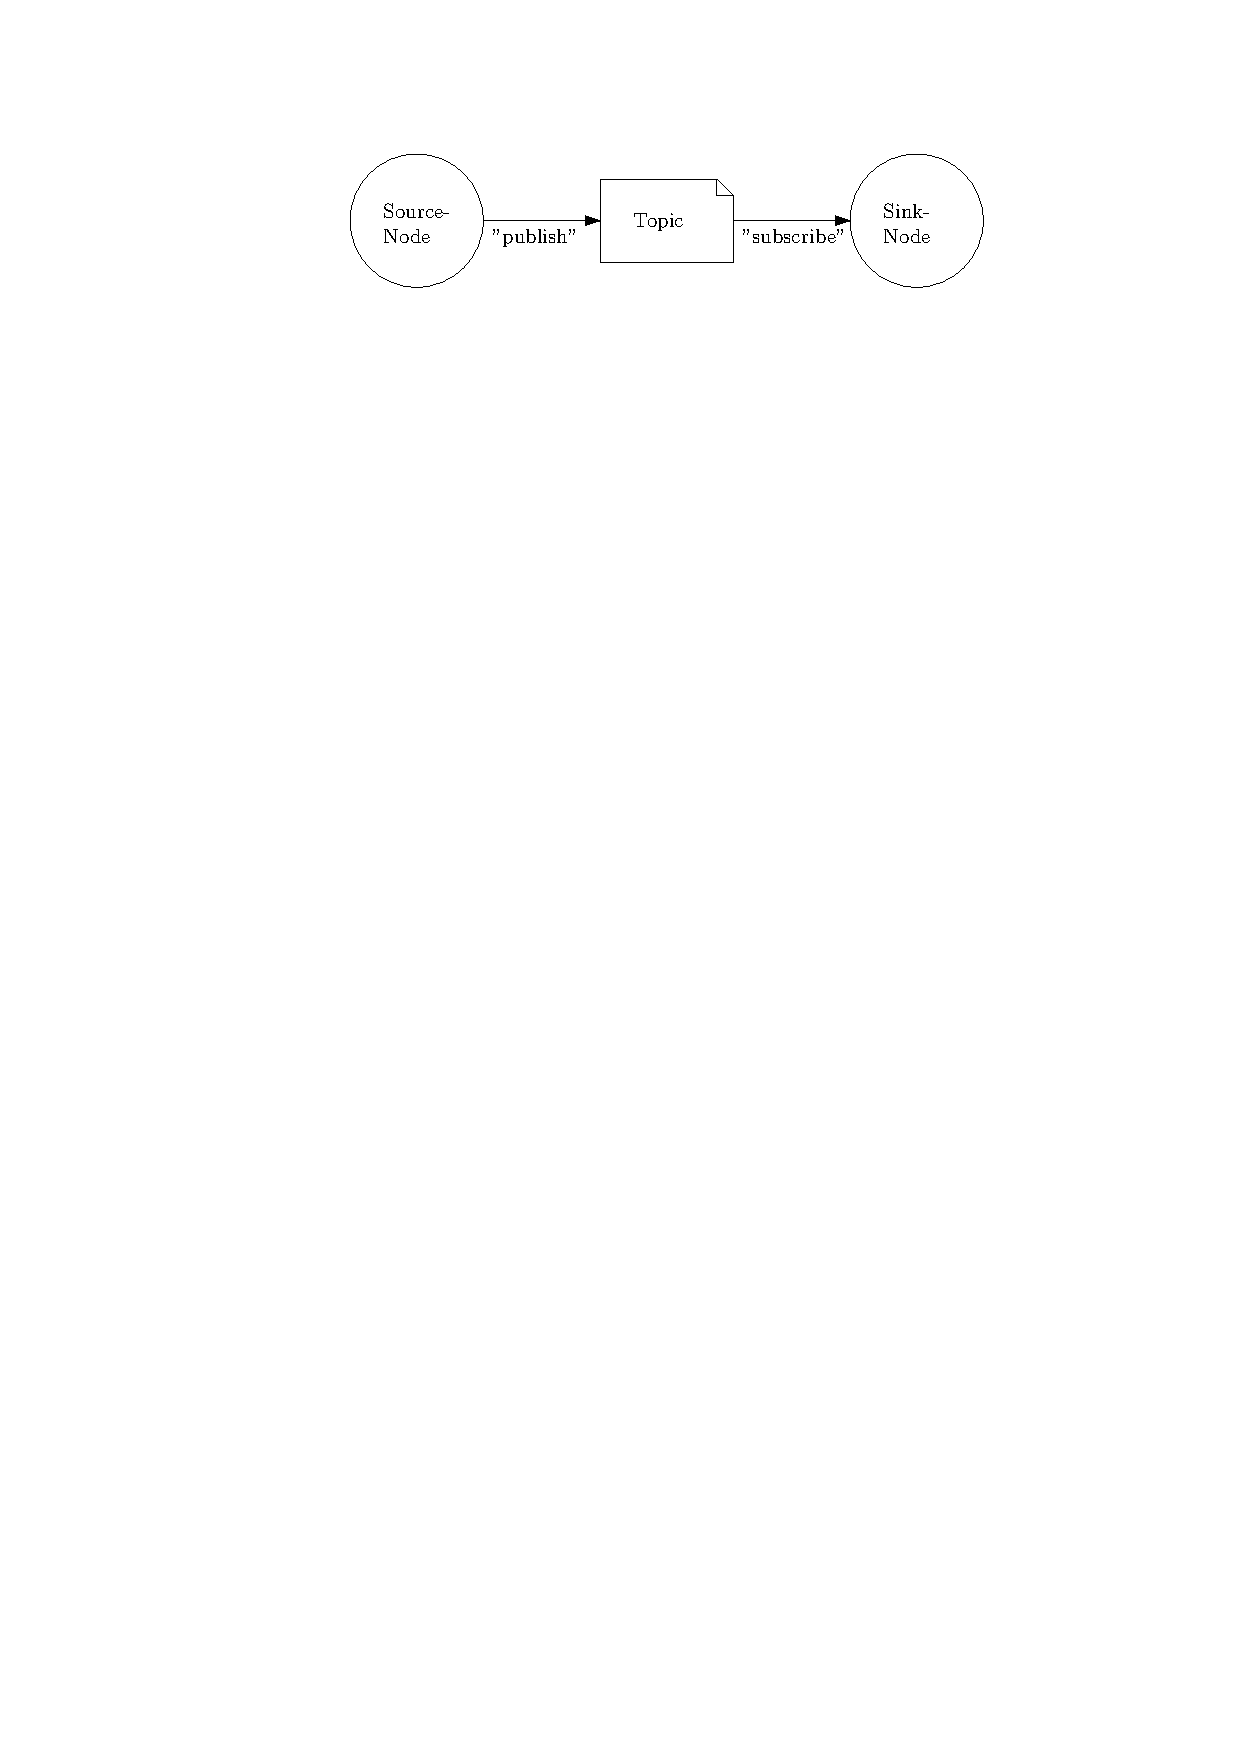
\includegraphics[width=0.6\textwidth]{./images/ros-topic.pdf}
		\label{fig:ros_topic}
	\end{figure}
	\item \textbf{Unidirektionale} Kommunikation
	\item \textbf{Punkt-zu-Punkt} und \textbf{Punkt-zu-vielen-Punkten}
\end{itemize}
\end{frame}
%%----------------------------------------------------------------------------------------
\begin{frame}{ROS Basics: Service}
\begin{alertblock}{Service ...}
... bezeichnet die bidirektionale Kommunikation zwischen zwei Nodes welche aus einem Service Request und einer Service Response bestehen.
\end{alertblock}
\begin{itemize}
	\item \textbf{Request} $\rightarrow$ $Node_1$ verlangt die Ausf\"uhrung eines Service von $Node_2$ (z.B. eine Addition)
	\item \textbf{Response} $\rightarrow$ $Node_2$ f\"uhrt den Service aus und returniert das Ergebnis an $Node_2$
	\begin{figure}[H]
		\centering
		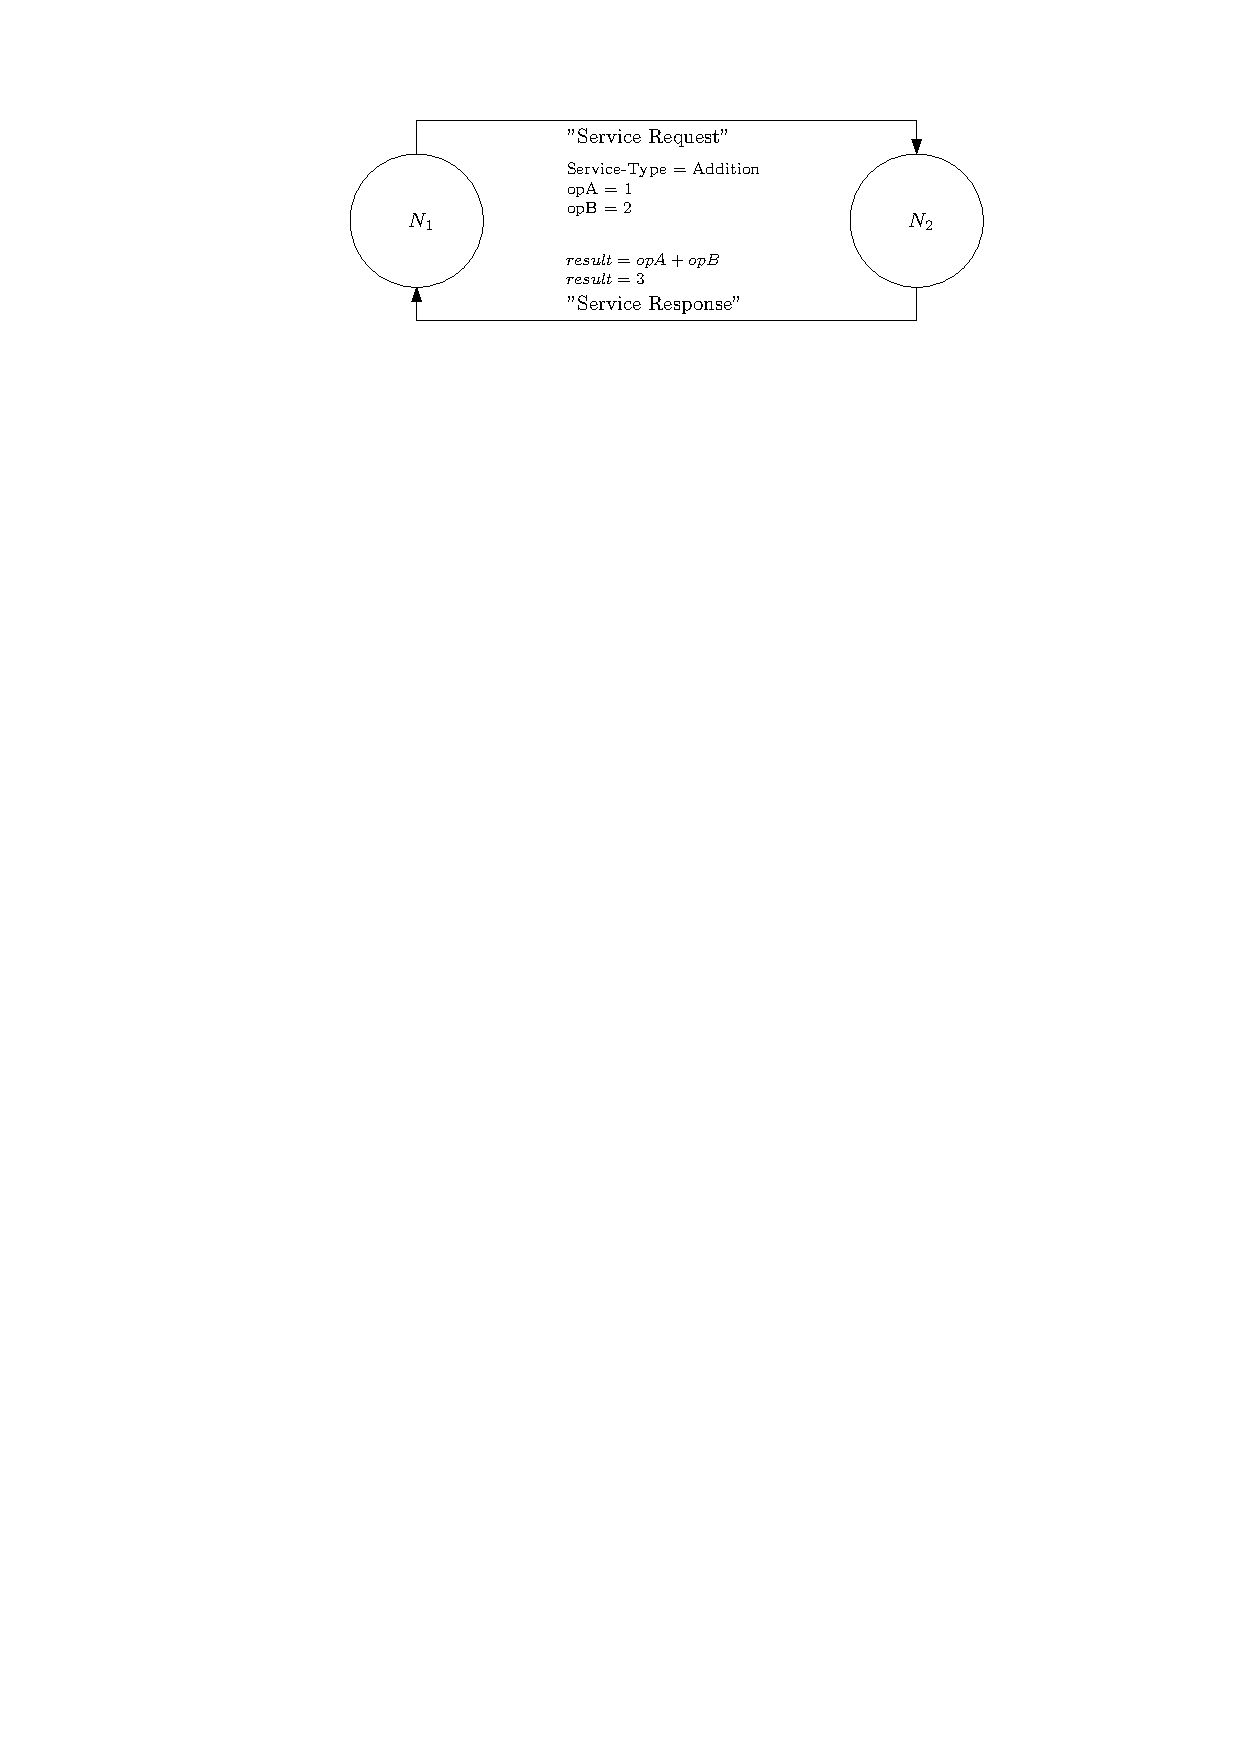
\includegraphics[width=0.6\textwidth]{./images/ros-service.pdf}
		\label{fig:ros_service}
	\end{figure}
	\item Konkrete Implementierung als \textbf{Remote Procedure Call}
	\item \textbf{Bidirektionale} Kommunikation
\end{itemize}
\end{frame}
%%----------------------------------------------------------------------------------------
\begin{frame}{ROS Basics: Zusammenfassung}
\begin{center}
\begin{huge}
ROS ist ein Framework welches einfache Interprozesskommunikation erm\"oglicht.
\end{huge}
\end{center}
\end{frame}
%%----------------------------------------------------------------------------------------
\begin{frame}{rosserial (1)}
\begin{alertblock}{rosserial ...}
... is a protocol for wrapping standard ROS serialized messages and multiplexing multiple topics and services over a character device such as a serial port or network socket.
\end{alertblock}
\begin{itemize}
	\item \textbf{rosserial erm\"oglicht die Kommunikation mit einem Arduino via Topics und Services}
\end{itemize}
\end{frame}
%%----------------------------------------------------------------------------------------
\begin{frame}{rosserial (2)}
	
\end{frame}
%%----------------------------------------------------------------------------------------
\begin{frame}{Conrad}
\begin{figure}[H]
	\centering
	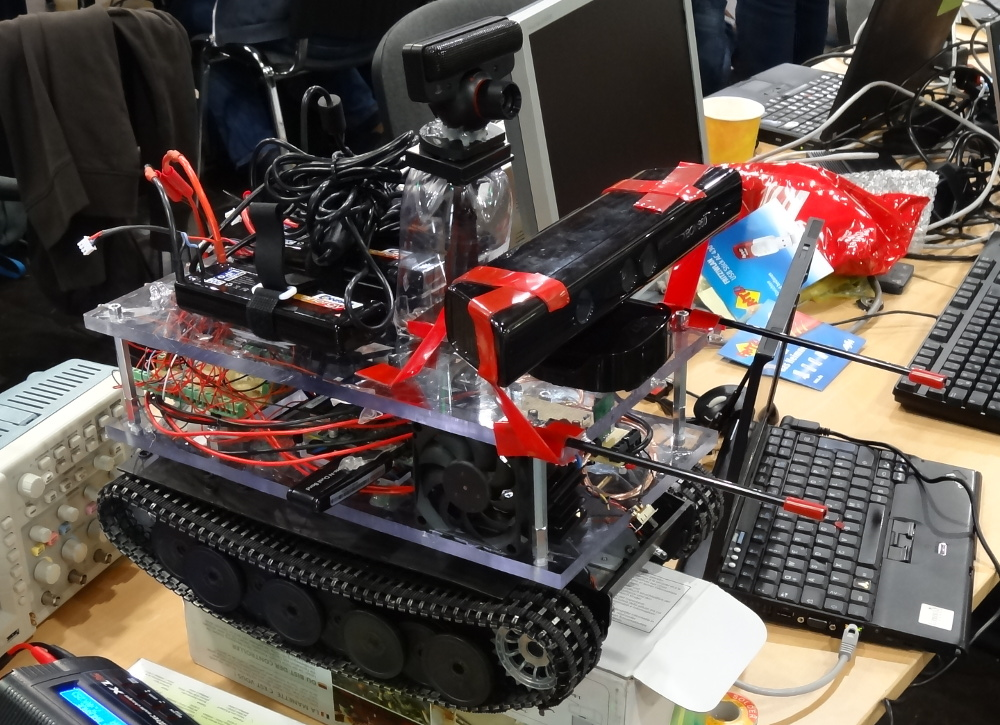
\includegraphics[width=0.5\textwidth]{./images/robot-conrad.jpg}
\end{figure}
\begin{itemize}
	\item \textbf{Motorsteuerung}: \url{https://github.com/AR2A/motor-controller-highpower-motorshield}
\end{itemize}
\begin{itemize}
	\item \textbf{Inertial Measurement Unit}: \url{https://github.com/AR2A/imu-minimu-arduino}
\end{itemize}
\end{frame}
%%----------------------------------------------------------------------------------------
\begin{frame}{Zusammenfassung}
\begin{large}F\"ur \textbf{kleine} Projekte:\end{large}
\begin{itemize}
	\item Arduino kann komplette Steuerung des Roboters \"ubernehmen
	\item Verwendung von Arduino als Vorlage f\"ur eigene Arduino basierte Platinen
\end{itemize}
\vspace{20px}
\begin{large}F\"ur \textbf{gro\ss{}e} Projekte:\end{large}
\begin{itemize}
	\item Arduino erm\"oglicht einem \"ubergeordneten Steuerungssystem den einfachen Zugriff auf Sensoren und Aktoren
	\item F\"ur Rapid-Prototyping (Arduino + Shield + Software)
	\item F\"ur professionelle L\"osung ist Entwicklung eigener Hard/Software notwendig
\end{itemize}
\end{frame}
%----------------------------------------------------------------------------------------
\begin{frame}
	\Huge{\centerline{Fragen}}
\end{frame}
%----------------------------------------------------------------------------------------
\begin{frame}[allowframebreaks]{Quellenverzeichnis}
\scriptsize{\bibliographystyle{ieeetr}}
\bibliography{references} %bibtex file name without .bib extension
\end{frame}
%----------------------------------------------------------------------------------------
\end{document} 
%----------------------------------------------------------------------------------------